\chapter{Visualizing Neural Networks}
\graphicspath{{figs/2b/}}

This exploration focuses on neural network visualization, a crucial aspect of understanding and analyzing how these models make decisions. It emphasizes the importance of interpretability and transparency in machine learning. Through the exploration of various visualization techniques, we can gain valuable insights into how these complex models interpret and process visual information. This endeavor helps bridge the divide between theoretical knowledge and real-world application, contributing to our deeper understanding of how neural networks function and their significance in modern AI solutions.

\section{Saliency Map}

This section focuses on identifying the most impactful pixels in an image for predicting its correct class. It employs a method proposed by \cite{simonyan2014deep}, which approximates the neural network around an image and visualizes the influence of each pixel.

\paragraph*{1. $ \bigstar $ Show and interpret the obtained results.}
In the process of visualizing multiple saliency maps, most of them exhibited consistent patterns, while some displayed inconsistencies. Let's examine each case.

% J'interprète souvent comme "le modèle regarde" alors que la saillancy map est que pour la class prédite et pas pour la ground truth faudrait visu les deux mais du coup pour limiter le nombre de figure mettre moins d'example ? 

In \Cref{fig:good_saliency_map}, we observe saliency maps that are generally consistent. When the model makes accurate predictions, we can observe high saliency values on the labeled object, i.e. it highlights only the important pixels. This makes it easy to recognize the images. This holds true for all the images in this figure, except for the fourth one where the model predicted "greenhouse" instead of "lakeside." In this case, the model did not focus on the lake boundaries, which led to the incorrect prediction. Instead, it primarily concentrated on the dark ground and the bright areas of the image, resulting in the "greenhouse" class prediction. 

In \Cref{fig:bad_saliency_map}, we encounter saliency maps that appear inconsistent. Both the first and fourth images are examples where the model's prediction is correct, but the corresponding saliency maps lack informativeness and appear blurry. In contrast, for the second and last images, the model seems to be focusing on the right regions, but it still predicts the wrong class.

\begin{figure}[H]
    \centering
    \begin{subfigure}{0.95\textwidth}
        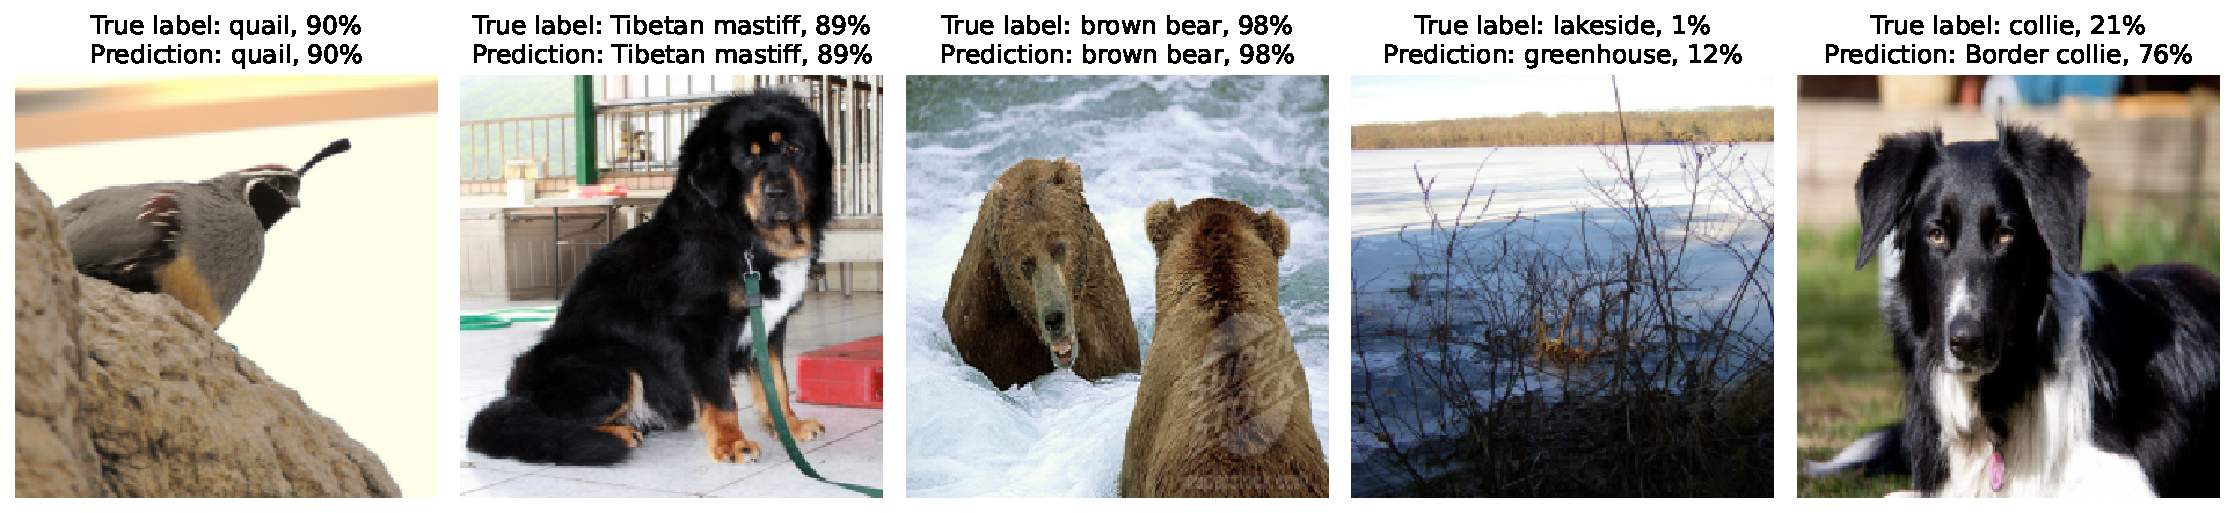
\includegraphics[width=\textwidth]{good_images}
        \caption{}
        \label{subfig:good_images1}
    \end{subfigure}
    \begin{subfigure}{0.95\textwidth}
        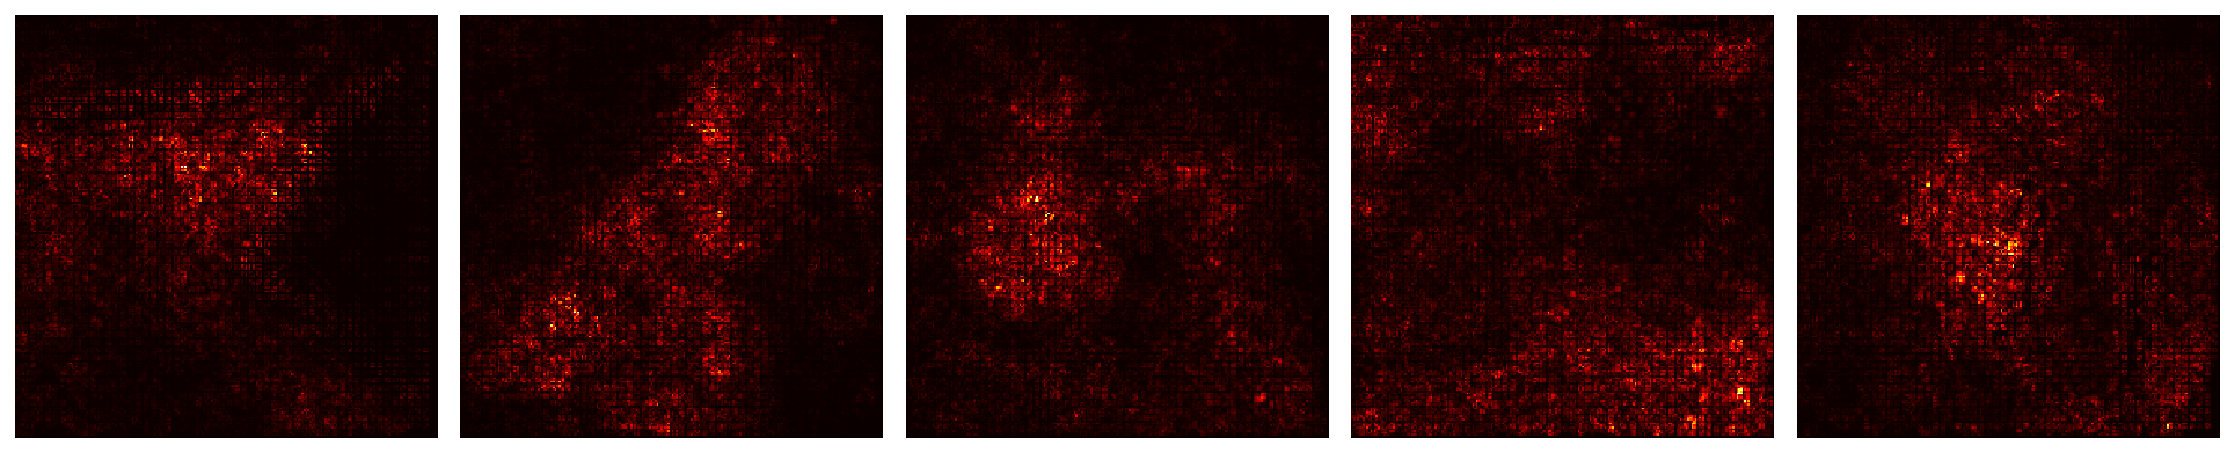
\includegraphics[width=\textwidth]{good_true_class_saliency}
        \caption{}
        \label{subfig:good_true_class_saliency}
    \end{subfigure}
    \begin{subfigure}{0.95\textwidth}
        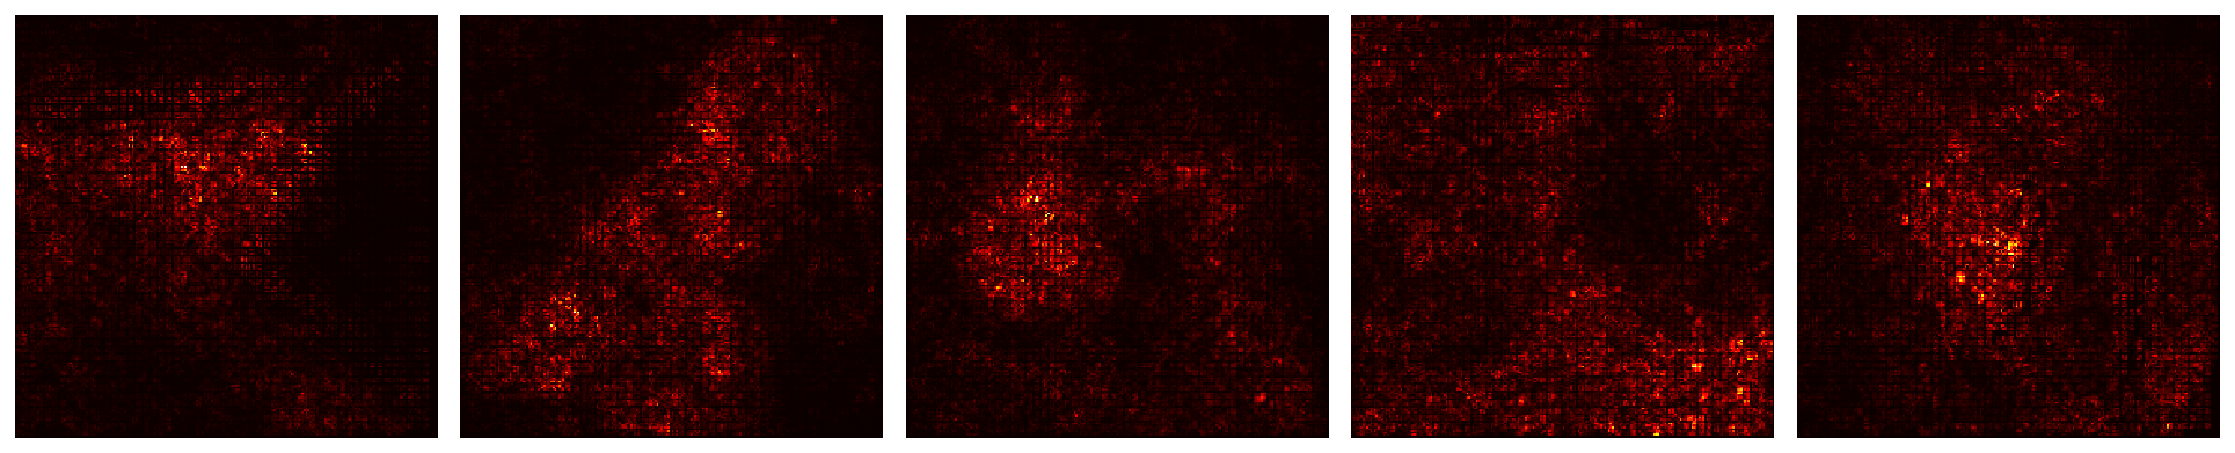
\includegraphics[width=\textwidth]{good_predicted_class_saliency}
        \caption{}
        \label{subfig:good_predicted_class_saliency}
    \end{subfigure}
    \caption{Illustration of (a) original images depicting the true label and predicted class by SqueezeNet, (b) saliency maps highlighting regions relevant to the true class, and (c) consistent saliency maps highlighting regions relevant to the predicted class.}
    \label{fig:good_saliency_map}
\end{figure}

%  In (a), the images display both the true label and the class predicted by the SqueezeNet model, providing insight into the model's performance. (b) visualizes regions in the images that contribute to the true class prediction, and (c) visualizes regions contributing to the predicted class, offering insights into the model's decision-making process.

\begin{figure}[H]
    \centering
    \begin{subfigure}{0.95\textwidth}
        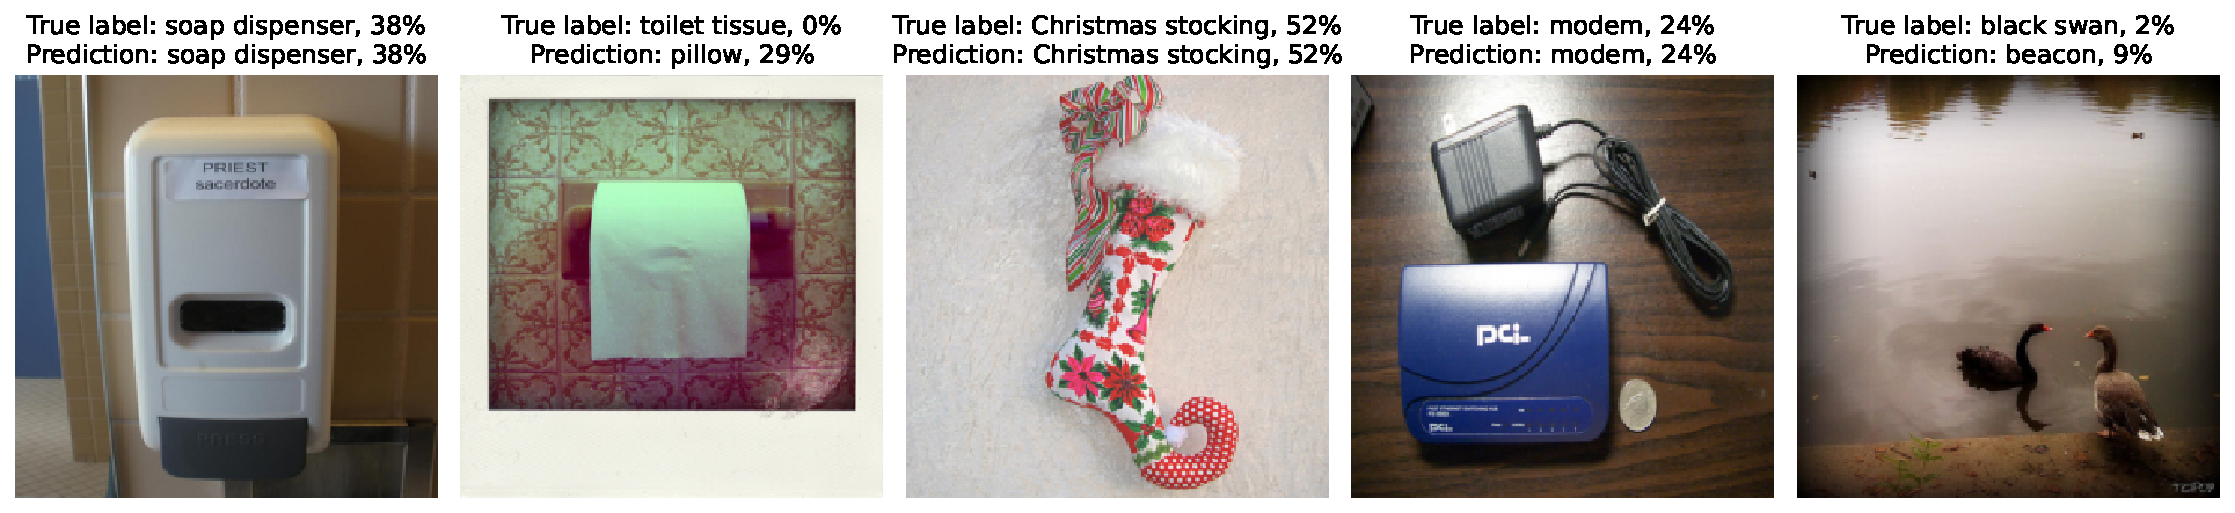
\includegraphics[width=\textwidth]{bad_images}
        \caption{}
        \label{subfig:bad_images}
    \end{subfigure}
    \begin{subfigure}{0.95\textwidth}
        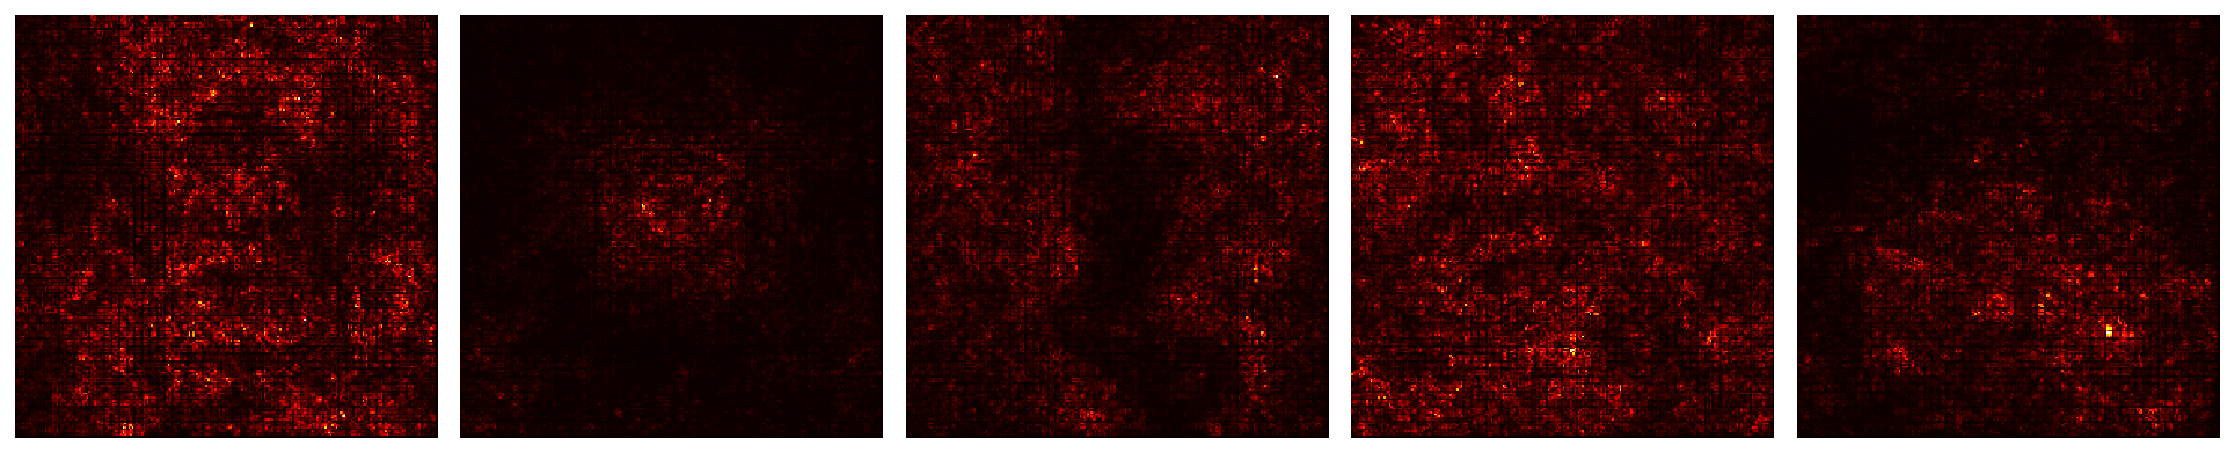
\includegraphics[width=\textwidth]{bad_true_class_saliency}
        \caption{}
        \label{subfig:bad_true_class_saliency}
    \end{subfigure}
    \begin{subfigure}{0.95\textwidth}
        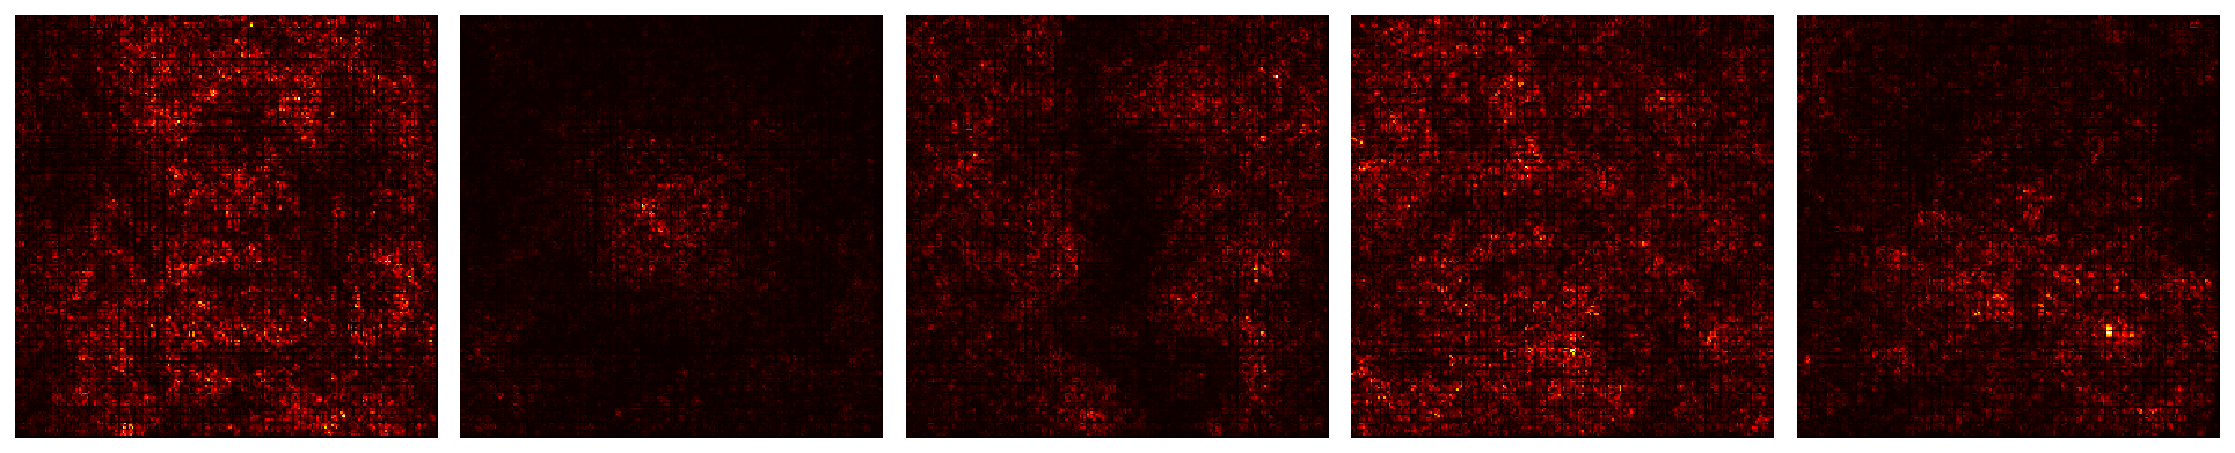
\includegraphics[width=\textwidth]{bad_predicted_class_saliency}
        \caption{}
        \label{subfig:bad_predicted_class_saliency}
    \end{subfigure}
    \caption{Illustration of (a) original images depicting the true label and predicted class by SqueezeNet, (b) saliency maps highlighting regions relevant to the true class, and (c) inconsistent saliency maps highlighting regions relevant to the predicted class.}
    \label{fig:bad_saliency_map}
\end{figure}

% figure où le modèle misclassify des images? nan on le fait déjà là

\paragraph*{2. Discuss the limits of this technique of visualization the impact of different pixels.}
As we discussed in the previous question, saliency maps can face challenges when dealing with images containing multiple objects or complex scenes. In such scenarios, these maps may become cluttered or unclear, making it challenging to extract the important pixels. They can also suffer from noise or, conversely, overemphasize certain features while downplaying others. This can result in a biased interpretation of the model's focus. Additionnaly, this technique (Vanilla Gradient) suffers from a saturation problem, as highlihted by \cite{shrikumar2019learning}. When ReLU is used, and when the activation goes below zero, it remains capped at zero and no longer change. This saturation issue may explain our previous observations regarding saliency maps. To address this problem, alternatives methods were subsequently introduced, such as SmoothGrad \citep{smilkov2017smoothgrad} and Grad-CAM \citep{Selvaraju_2019}.

As with most explanation methods, interpreting saliency maps can be subjective, especially when they are ambiguous. Different individuals may draw different conclusions from the same saliency map, resulting in inconsistent interpretations of the model's behavior. This underscores the challenge of determining whether or not an explanation is correct. To gain a better understanding, we found it necessary to repeatedly analyze and visualize various saliency maps, particularly when they exhibited inconsistencies. It can be a complex task to keep in mind that each map represents the model's attention for a specific class, not the entire model. Examining saliency maps for other high-probability classes can provide additional context, contributing to a more complete understanding of the model's decision-making process. 

It's important to note that saliency maps tend to highlight correlations rather than establishing causation. They reveal areas where the model directed its attention but do not necessarily imply that these areas directly influenced the model's decision.

\paragraph*{3. Can this technique be used for a different purpose than interpreting the network?}

Saliency maps can be used to identify and localize important objects or regions in an image. They can find applications in image segmentation, for instance in applications like automated image tagging or initial steps of object detection. This can also help to create more effective augmented images by applying transformations (like rotations, scaling, cropping) that preserve these key areas. This technique is primarily suited for image data. Its utility is limited in non-visual domains or for models that integrate multiple types of data (like text and images).

%Feature Engineering and Selection: By identifying which parts of an input are most salient to a model's decision, saliency maps can inform feature engineering and selection in machine learning. This can be particularly useful in fine-tuning models by focusing on the most relevant features. ??????

\paragraph*{4. \textbf{Bonus:} Test with a diffrentent network, for example VGG16, and comment.} \label{paragraph:bonus_VGG}
% Guillaume a fait sur un ViT aussi
% Make a comparaison plot for most of the "bad" saliency map (ie no more missclassif for example), much better frontier, better classification also, Tibetan mastiff dog much clear frontiere too 

We generated saliency maps using VGG16 on the same examples. Notably, we observed that there were no misclassifications due to VGG16's superior image classification capabilities. Consequently, the saliency maps are much better! They exhibited notable improvements, featuring reduced noise and more precise object boundaries compared to those produced with SqueezeNet.

This outcome highlights the impact of the choice of neural network architecture on the effectiveness of saliency map generation. VGG16's strong performance in image classification results in more reliable and visually coherent saliency maps, making it a favorable choice for tasks that rely on accurate attention mapping within images.

% \begin{figure}[H]
%     \centering
%     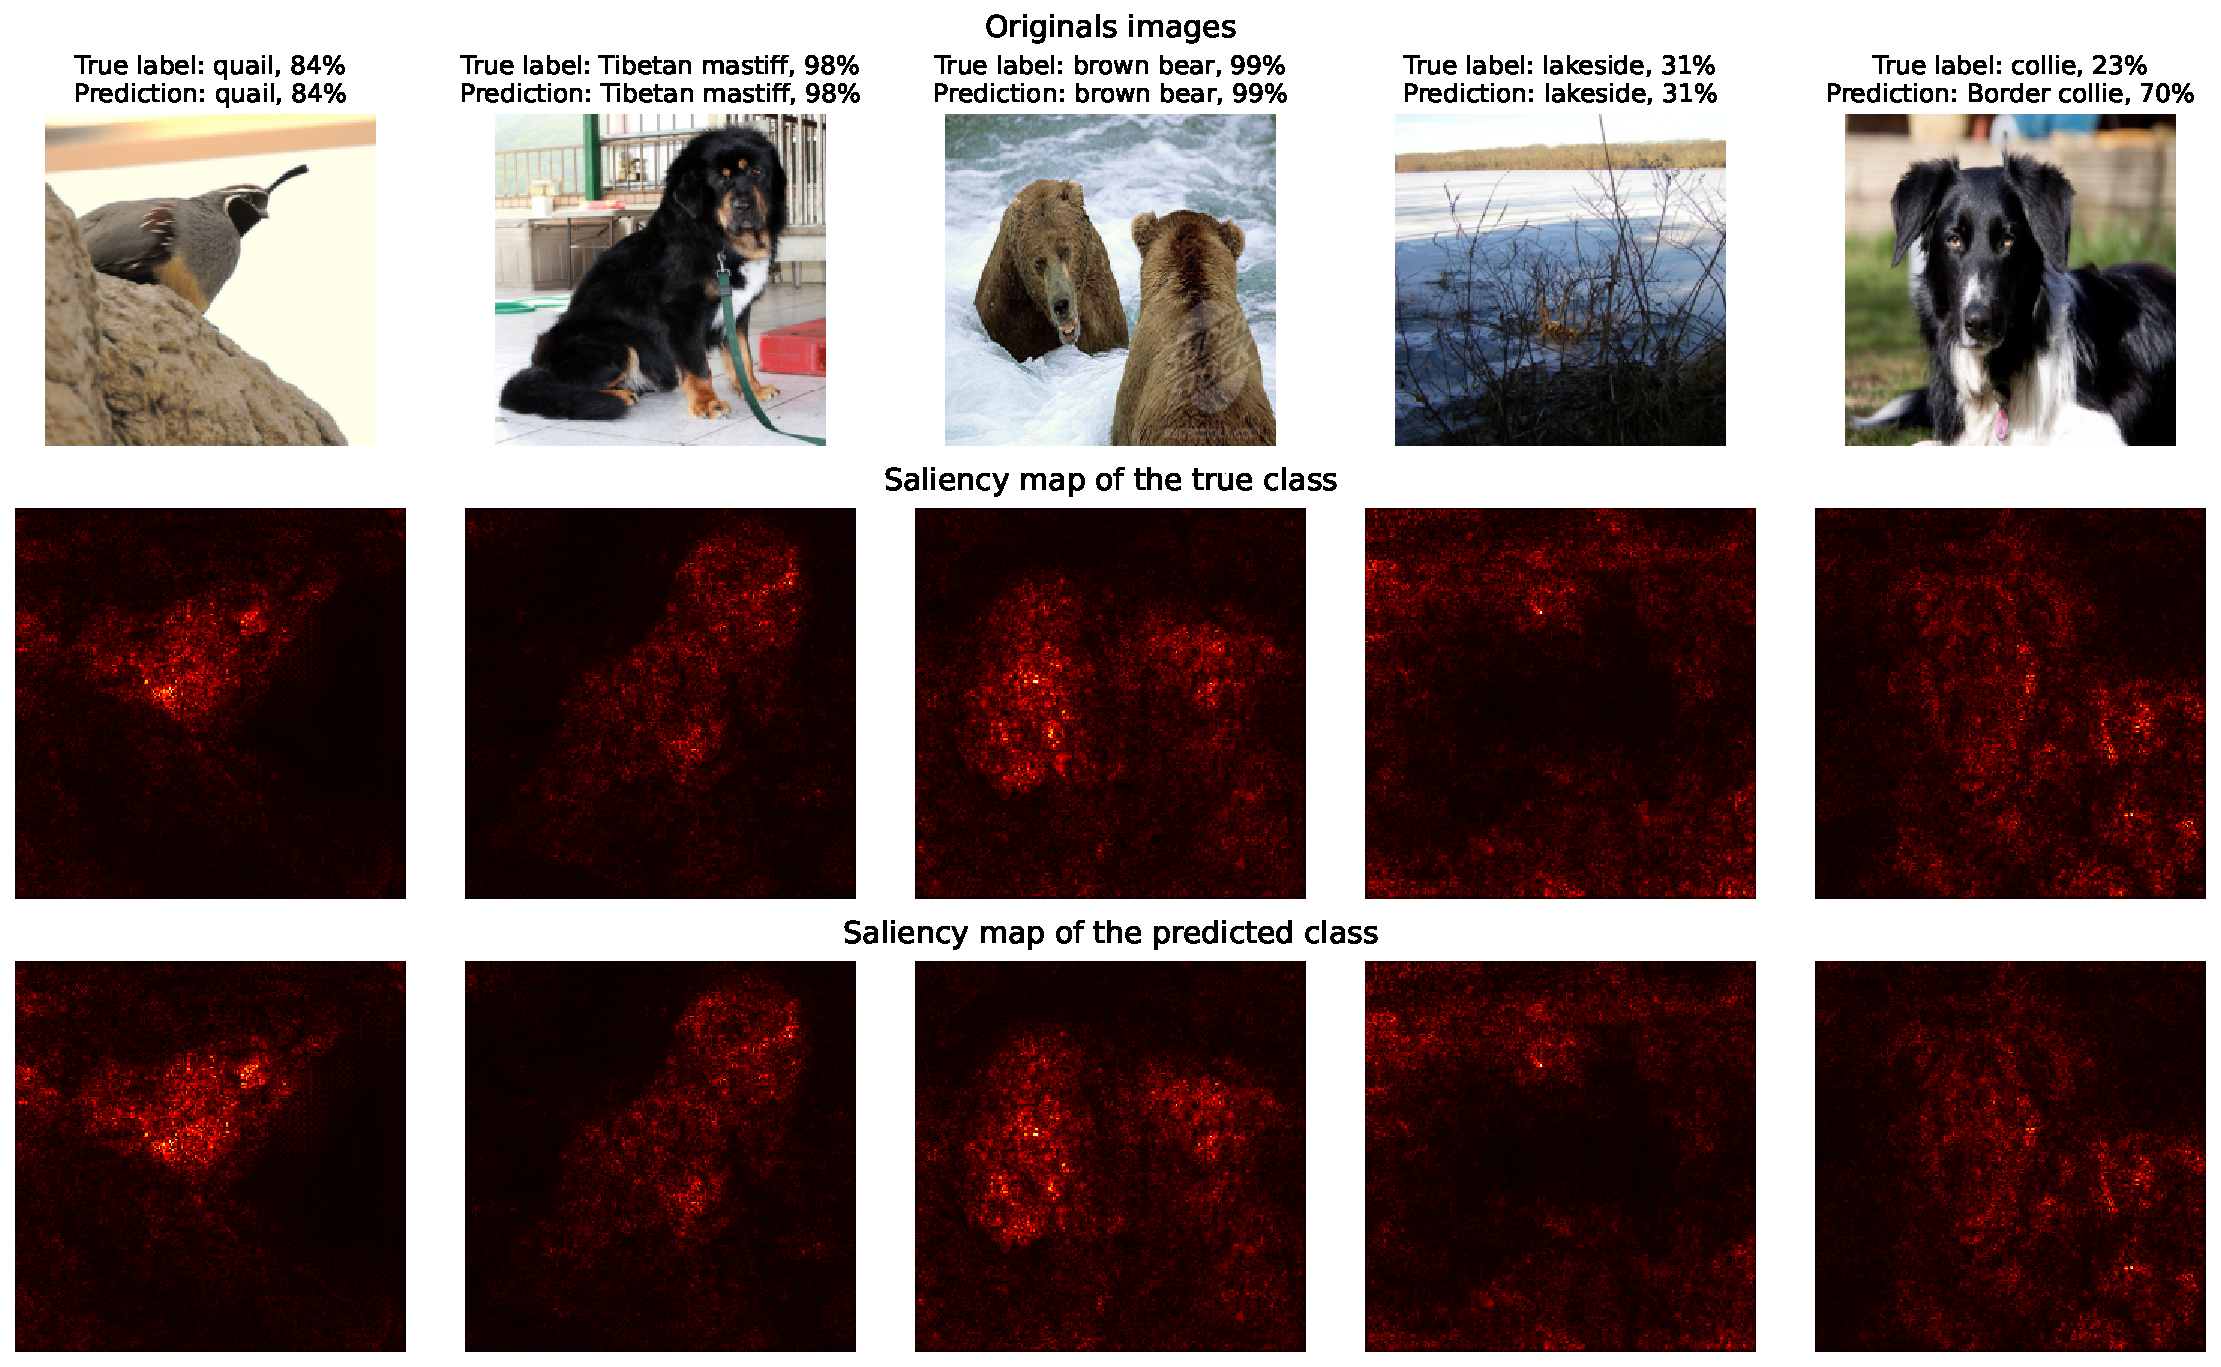
\includegraphics[width=.9\textwidth]{good_saliency_map_vgg16.pdf}
%     \caption{Consistent saliency maps of the predicted class}
%     \label{fig:good_saliency_map_vgg16}
% \end{figure}

\begin{figure}[H]
    \centering
    \begin{subfigure}{0.95\textwidth}
        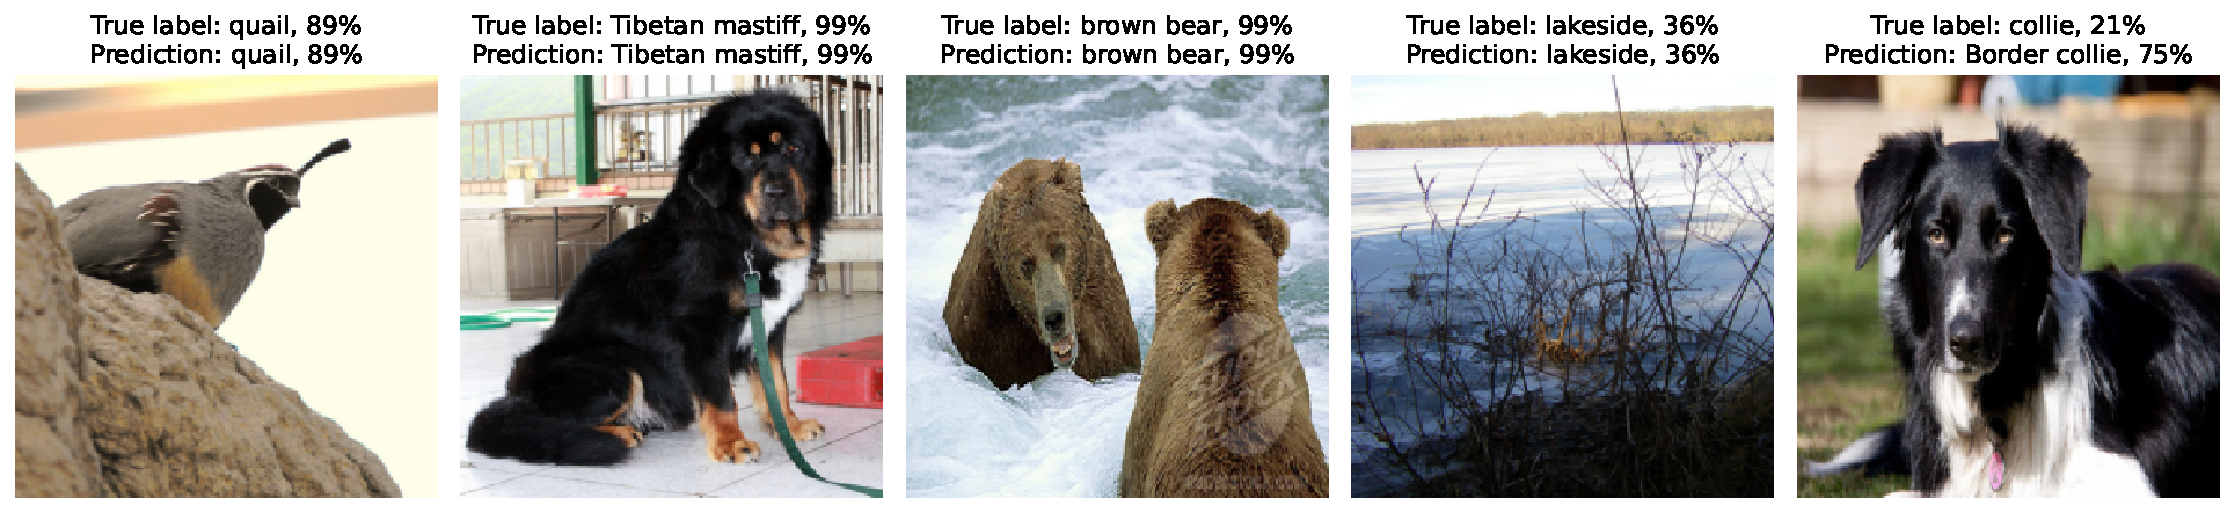
\includegraphics[width=\textwidth]{good_images_vgg16}
        \caption{}
        \label{subfig:good_images_vgg16}
    \end{subfigure}
    \begin{subfigure}{0.95\textwidth}
        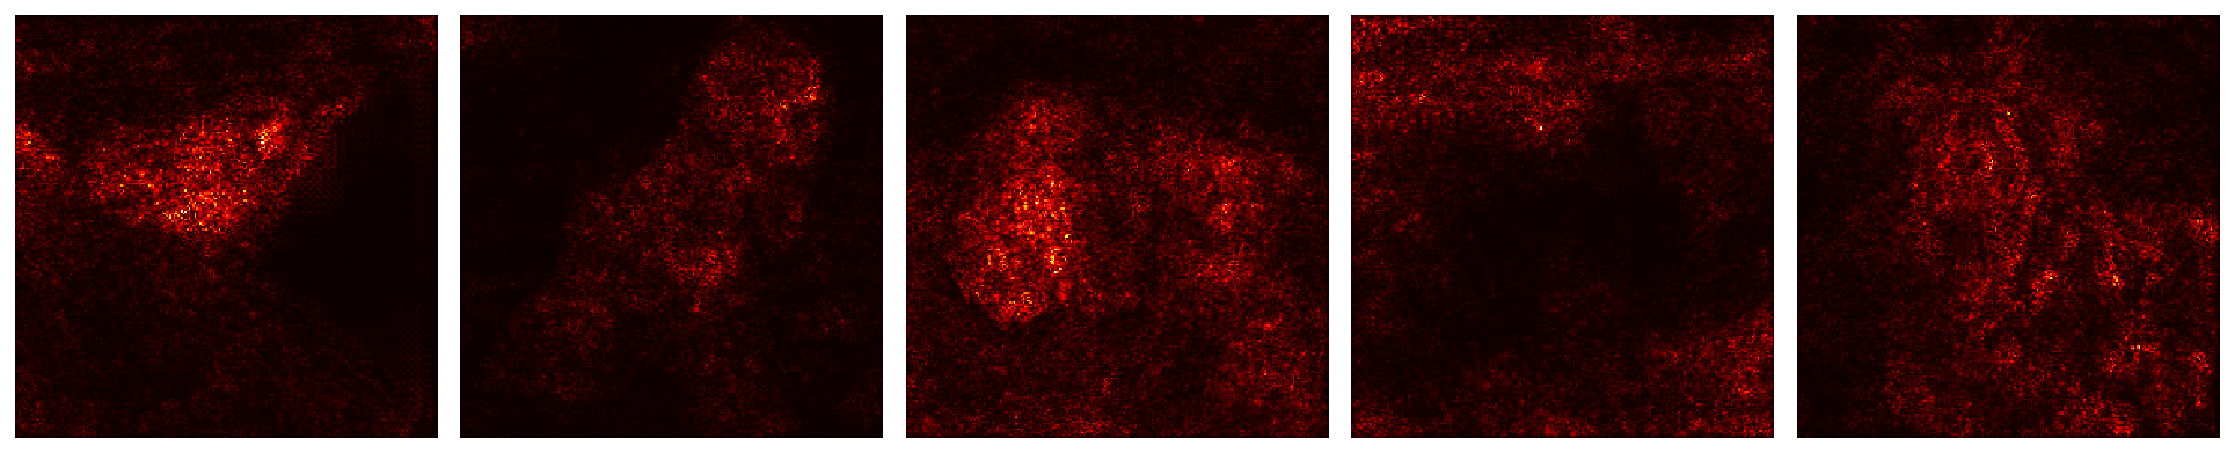
\includegraphics[width=\textwidth]{good_true_class_saliency_vgg16}
        \caption{}
        \label{subfig:good_true_class_saliency_vgg16}
    \end{subfigure}
    \begin{subfigure}{0.95\textwidth}
        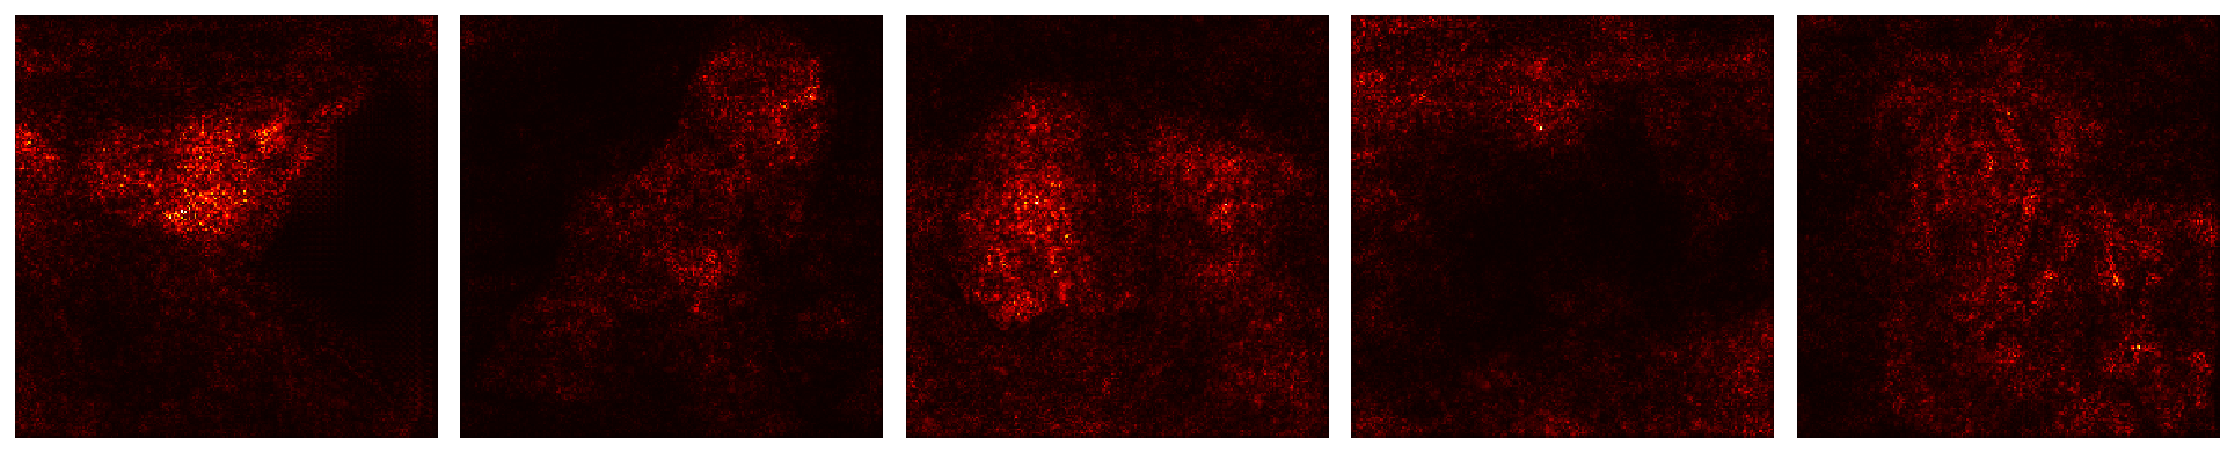
\includegraphics[width=\textwidth]{good_predicted_class_saliency_vgg16}
        \caption{}
        \label{subfig:good_predicted_class_saliency_vgg16}
    \end{subfigure}
    \caption{Illustration of (a) original images depicting the true label and predicted class by VGG16, (b) saliency maps highlighting regions relevant to the true class, and (c) consistent saliency maps highlighting regions relevant to the predicted class.}
    \label{fig:good_saliency_map_vgg16}
\end{figure}

% \begin{figure}[H]
%     \centering  
%     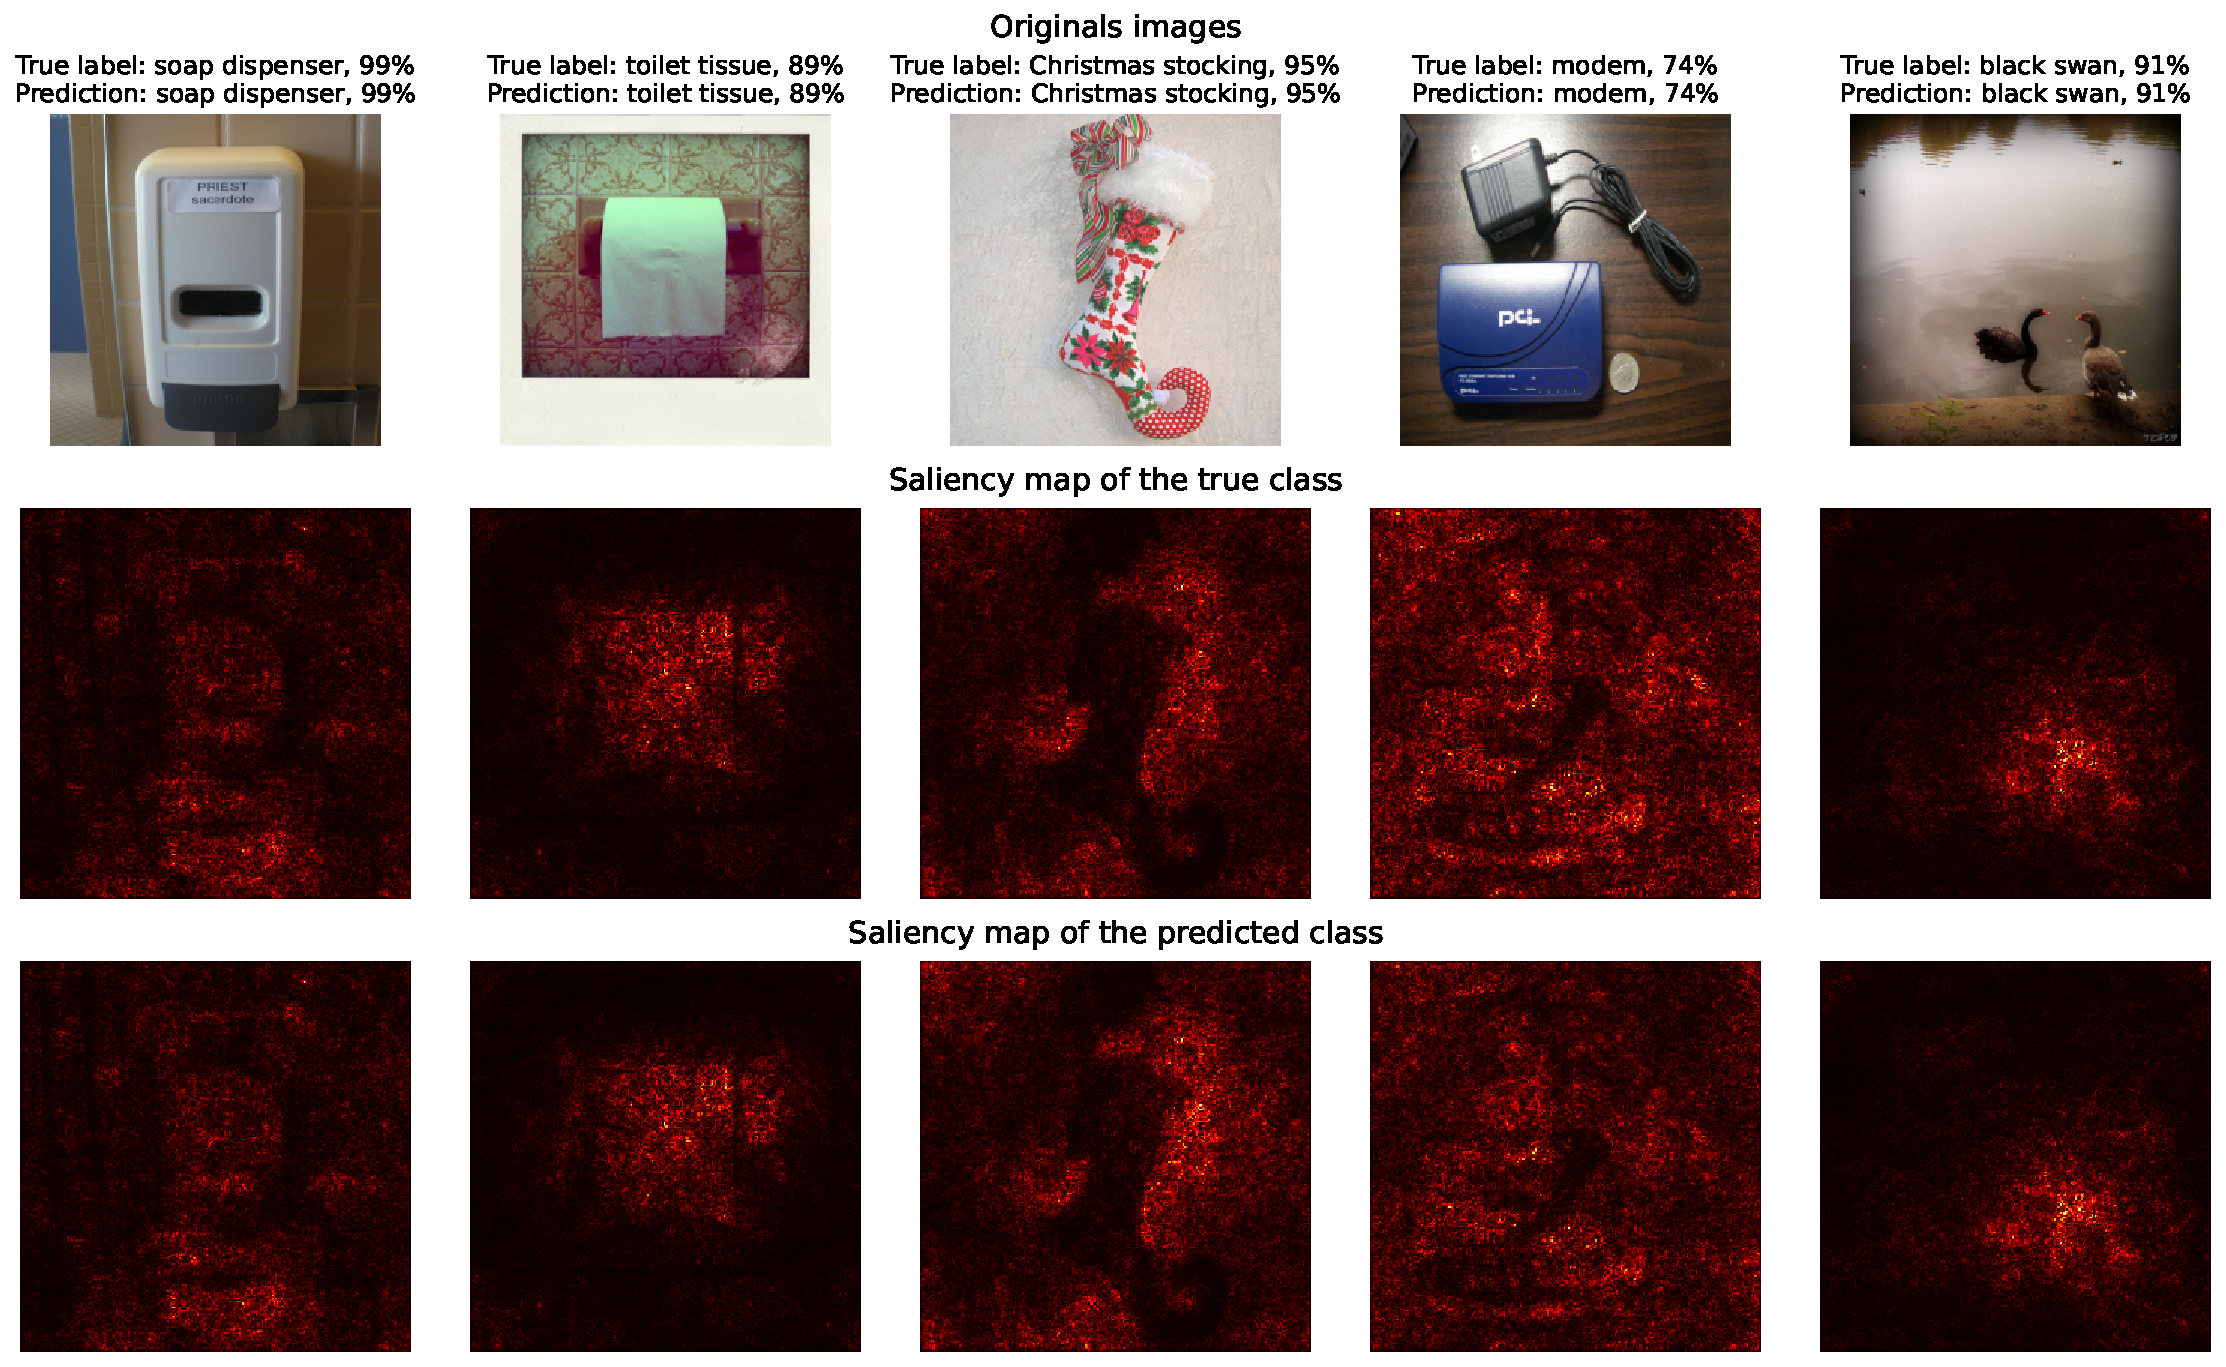
\includegraphics[width=.9\textwidth]{bad_saliency_map_vgg16.pdf}
%     \caption{Inconsistent saliency maps of the predicted class}
%     \label{fig:bad_saliency_map_vgg16}
% \end{figure}

\begin{figure}[H]
    \centering
    \begin{subfigure}{0.95\textwidth}
        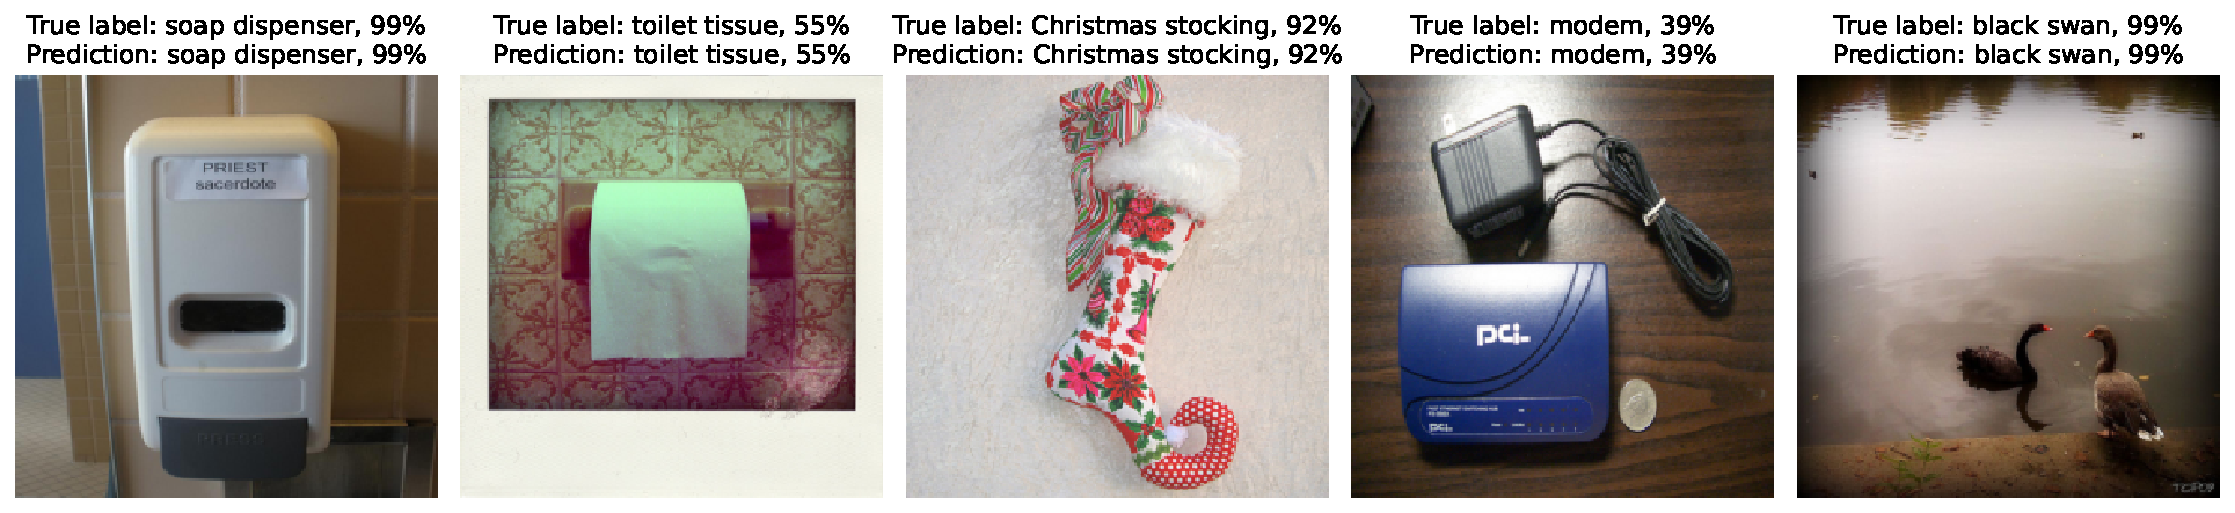
\includegraphics[width=\textwidth]{bad_images_vgg16}
        \caption{}
        \label{subfig:bad_images_vgg16}
    \end{subfigure}
    \begin{subfigure}{0.95\textwidth}
        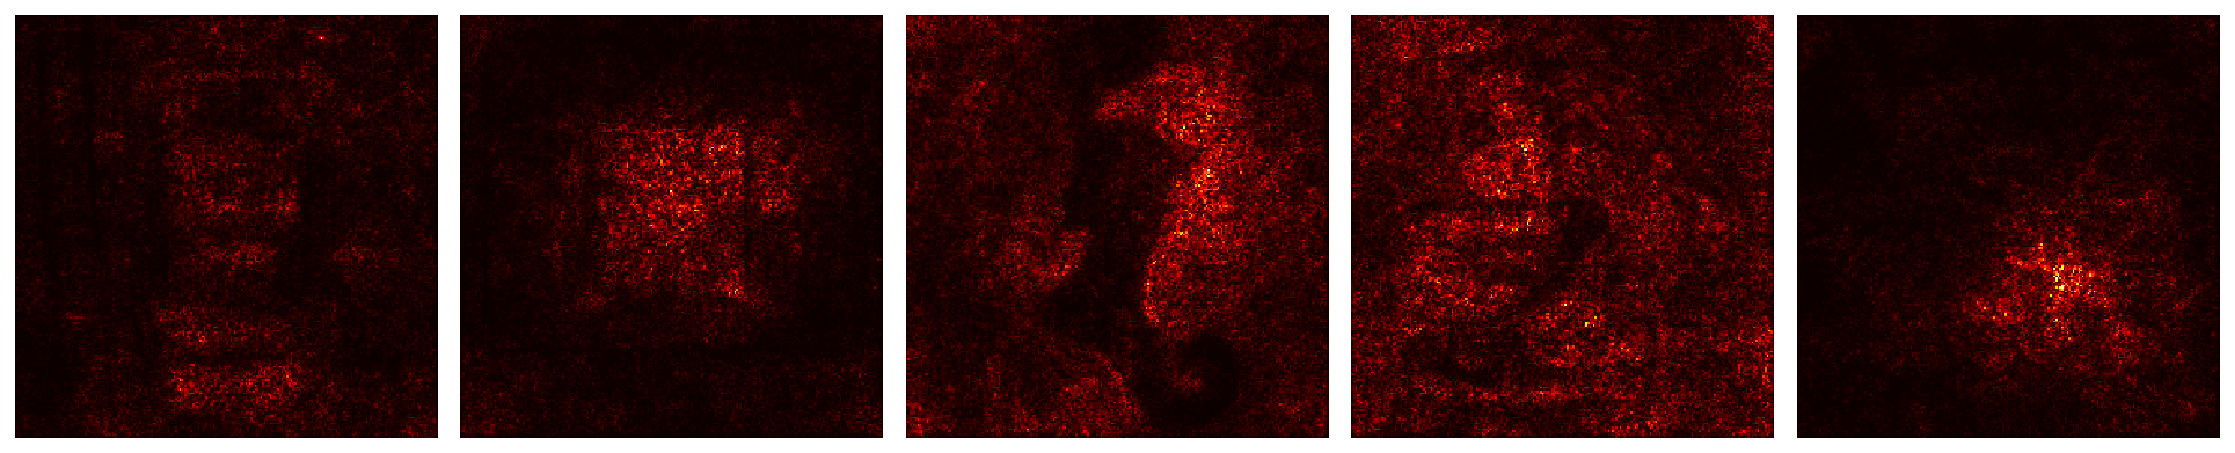
\includegraphics[width=\textwidth]{bad_true_class_saliency_vgg16}
        \caption{}
        \label{subfig:bad_true_class_saliency_vgg16}
    \end{subfigure}
    \begin{subfigure}{0.95\textwidth}
        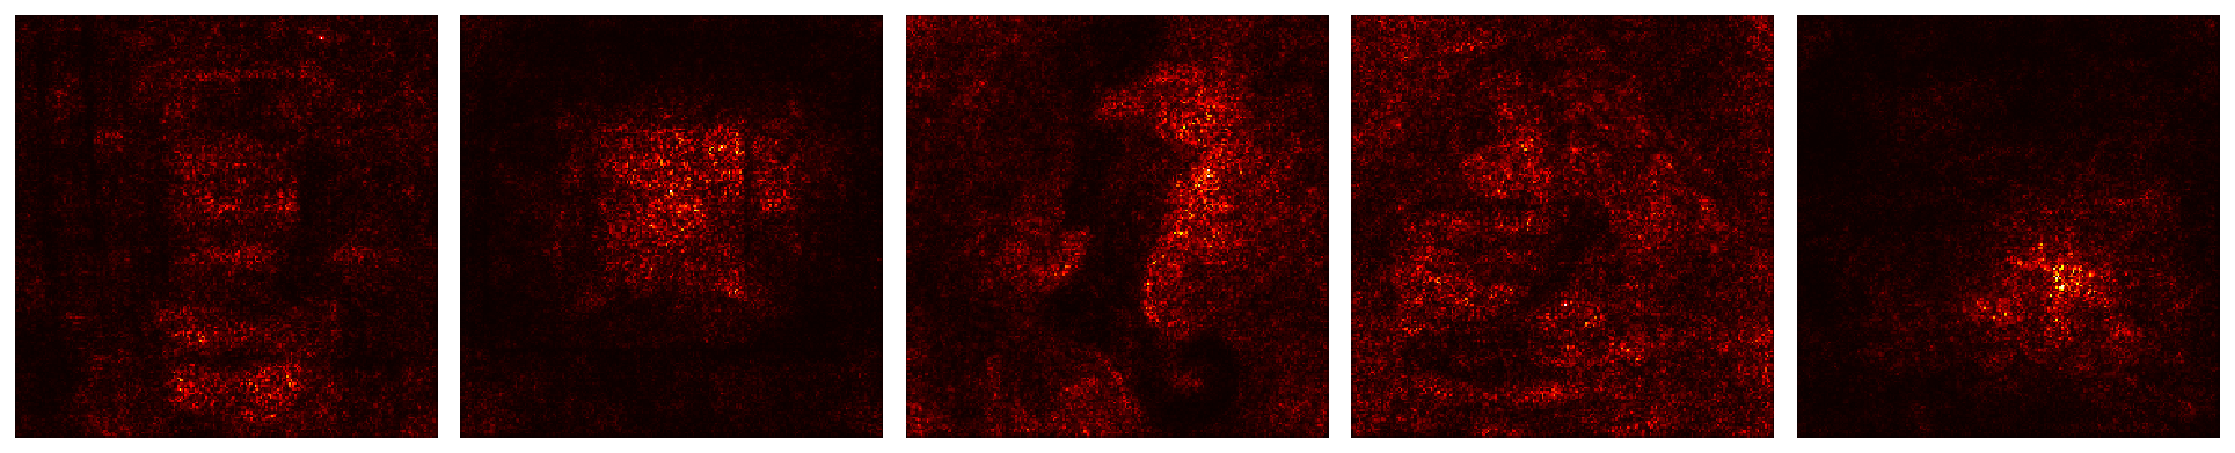
\includegraphics[width=\textwidth]{bad_predicted_class_saliency_vgg16}
        \caption{}
        \label{subfig:bad_predicted_class_saliency_vgg16}
    \end{subfigure}
    \caption{Illustration of (a) original images depicting the true label and predicted class by VGG16, (b) saliency maps highlighting regions relevant to the true class, and (c) consistent saliency maps highlighting regions relevant to the predicted class.}
    \label{fig:bad_saliency_map_vgg16}
\end{figure}


\section{Adversarial Example}

Here, the goal is to study the vulnerability of CNNs to minor, imperceptible modifications in an image that lead to misclassification. This concept, introduced by \cite{szegedy2014intriguing}, reveals the limitations and unexpected behaviors of neural networks. Adversarial examples can be compared to counterfactual examples used in common artificial intelligence explainability methods, but their purpose is to deceive the model rather than interpret it.

\paragraph*{5. $ \bigstar $ Show and interpret the obtained results.}

In the part of the pratical, we created adversarail example. We apply imperceptible, slight and carefully calculated modifications to the input image such that it is misclassified by a neural network. This is done by applying gradient backpropagation to find out how to tweak the pixel values of the original image so as to change the network's prediction. The adjustments are made according to the gradient of the loss with respect to the input image, and the process iteratively continues until the image is misclassified.

Our results are presented in \Cref{fig:adv_exmp}. The right column present original image, before any intervention, the left column the modified misclassified image, and in the middle column, the magnified difference (10x) between them. Despite the visual similarity of the two images on either side, the neural network classifies them as two different breeds due to the small, calculated changes that showed in the center image.

Interpreting this result, it's clear that even minimal changes that are imperceptible or nearly imperceptible to humans can lead to misclassification by an AI. This demonstrates the fragility of neural networks to adversarial attacks and underscores the importance of understanding and defending against such manipulations, especially in applications where security and reliability are crucial.

Adversarial examples and techniques have practical applications beyond academic interest, particularly in enhancing privacy and countering mass surveillance. For instance, \href{https://www.capable.design}{Cap\_able's Manifesto Collection} is a clothing line that uses patterns designed to shield facial recognition technologies. These garments are not recognized by models such as Yolo, instead causing misidentifications as various animals or inanimate objects. This line of clothing opens up a discussion on privacy and the protection of individuals from the misuse of biometric recognition cameras, offering a way to defend against unlawful intrusion into personal data and safeguard fundamental rights in public spaces.

\begin{figure}[p]
    \centering
    \begin{subfigure}[b]{\textwidth}
        \centering
        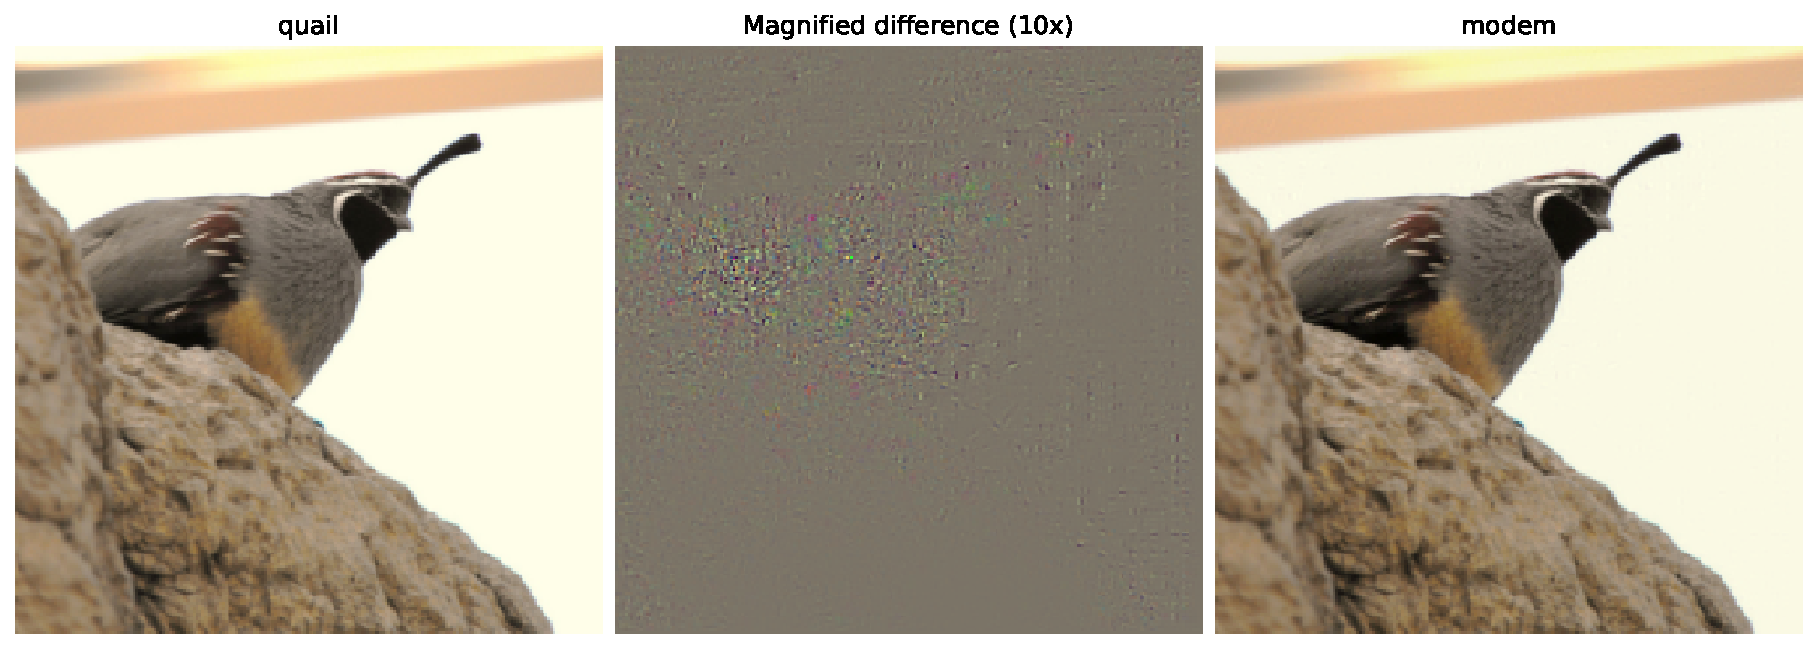
\includegraphics[width=.95\linewidth]{figs_propre2/adv_exmp.pdf}
        \label{fig:adv_exmp:sub1}
    \end{subfigure}
    
    \begin{subfigure}[b]{\textwidth}
        \centering
        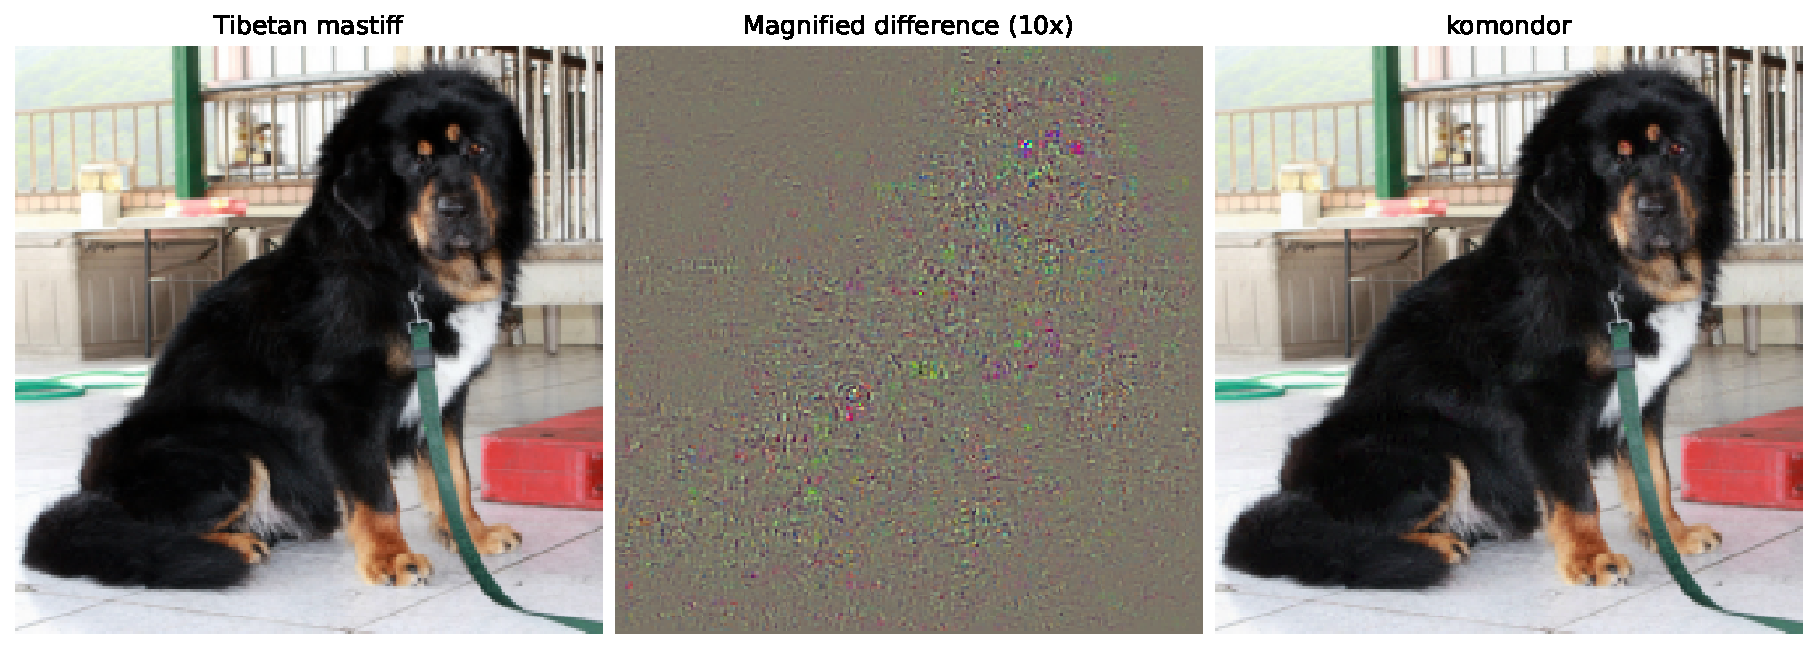
\includegraphics[width=.95\linewidth]{figs_propre2/adv_exmp2.pdf}
        \label{fig:adv_exmp:sub2}
    \end{subfigure}

    \begin{subfigure}[b]{\textwidth}
        \centering
        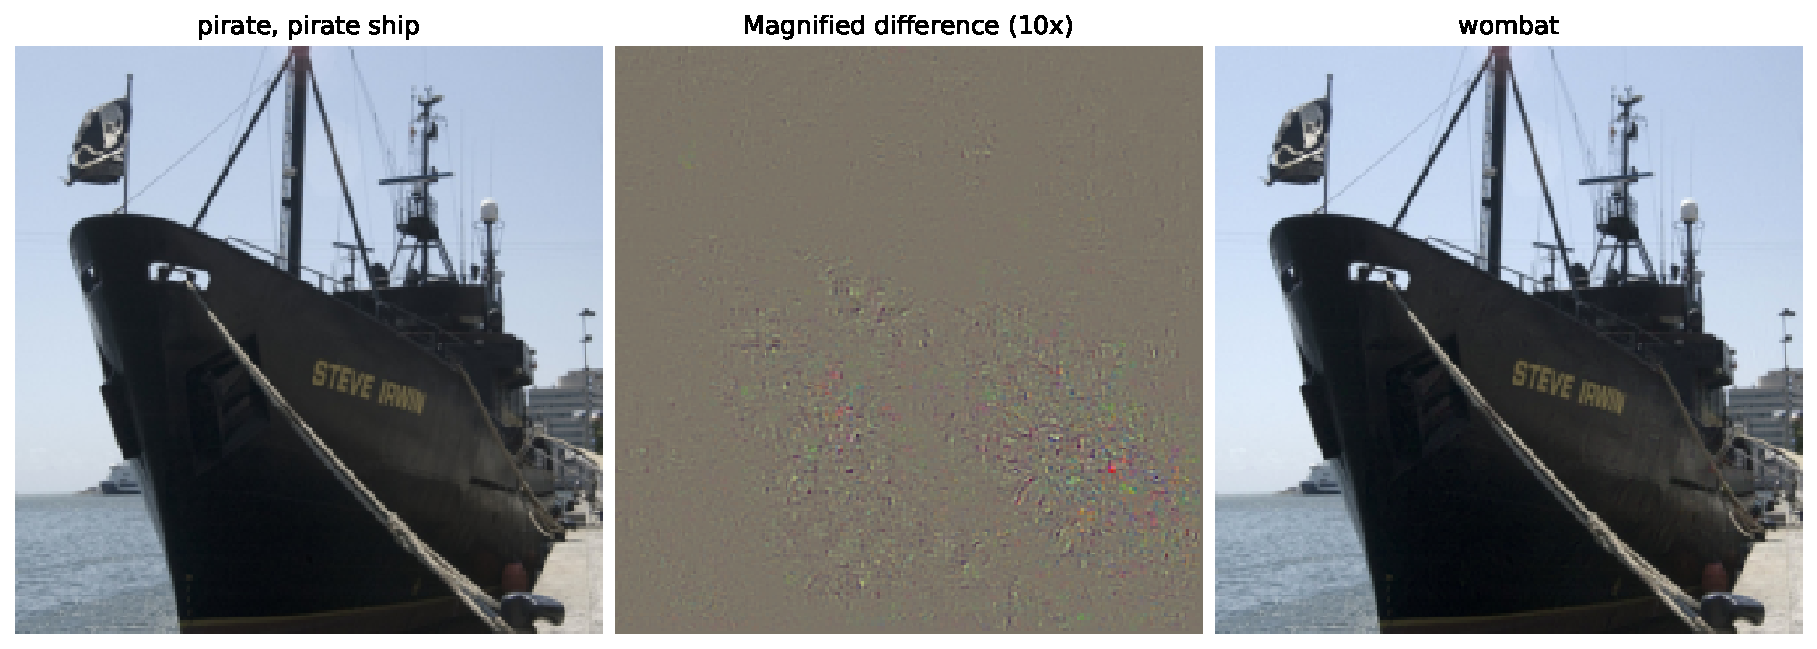
\includegraphics[width=.95\linewidth]{figs_propre2/adv_exmp3.pdf}
        \label{fig:adv_exmp:sub3}
    \end{subfigure}
    \caption{Adversarial examples. The right column displays the original image, the middle column shows the magnified difference added to the original image to deceive the model, and the left column presents the image that successfully fools the model.}
    \label{fig:adv_exmp}
\end{figure}

% une observation à faire c'est : plus un modèle est sûr de sa prédi, plus il faudra faire d'itérations pour le tromper, et vice-versa.

\paragraph*{6. In practice, what consequences can this method have when using convolutional neural networks?}

For example, consider the ability to trick a model into misclassifying a banana as a toaster using a printable label, as demonstrated by \cite{brown2018adversarial}. While this may seem like a playful experiment, it raises significant concerns when applied to critical domains like autonomous vehicles or medical imaging. 

Although our method requires access to model parameters, \cite{athalye2018synthesizing} has shown that it's possible to perform an adversarial attack without such access, known as a black-box attack. Consequently, an attacker could potentially deceive autonomous vehicles into making hazardous decisions, such as veering into another lane or perceiving non-existent information—incidents that have already occurred. 

This method has the potential to be exploited by malicious individuals to intentionally mislead a model, particularly as machine learning models become increasingly integrated into systems. As a result, this topic becomes a serious concern in the realm of cybersecurity, leading to an arms race between attackers and defenders to safeguard against such vulnerabilities.

\paragraph*{7. \textbf{Bonus:} Discuss the limits of this naive way to construct adversarial images. Can you propose some alternative or modified ways? (You can base these on recent research)}

% limits ??
One major limit of this naive way is that it requires many pixels to be changed. This led to the question: is it possible to deceive a neural network by modifying only one pixel? \cite{Su_2019} demonstrated that it is actually possible.

This method was inspired by biological evolution studies, and uses differential evolution to determine which to modify and how. It starts with a population of candidate solutions, each representing a potential pixel modification encoded by a five-element vector (coordinates and RGB values). The process then generates new generations of candidates (children) from the existing ones (parents) using a specific formula that involves mixing attributes from three random parent pixels. The process aims to find an adversarial example that causes the classifier to misidentify the image. It continues until such an example is found or until it reaches a user-specified iteration limit.

\section{Class Visualization}

This section aims to generate images that highlight the type of patterns detected by a network for a particular class, based on techniques developed by \cite{simonyan2014deep} and \cite{yosinski2015understanding}. This method helps in visualizing what features the network prioritizes for classification. To view the animated visuals in this section, you can use Adobe Acrobat Reader or access them from a separate folder provided with the materials.

\paragraph*{8. $ \bigstar $ Show and interpret the obtained results.}
Class visualization is a technique aimed at understanding what features or patterns a CNN has learned to recognize for a specific class. It involves generating an input image that maximally activates a class score in the network. Here, we've done this by iteratively modifying an initial random image to increase the activation of the desired class through gradient ascent on the class score with respect to the input image.

As a first try of this method, we decided to visualize our prefered animal: a wombat. \Cref{fig:class_viz_wombat} present a class visualization for a wombat after 1000 epochs and using the default regularization parameters in the given implementation (regularization factor of $10^{-3}$, bluring every ten epoch, learning rate of $5$). While examining some of our animations, we observed the occurrence of blurring every 10 steps.

Interpretation: The reason the figure appears as it does, featuring multiple, somewhat distorted wombats and a somewhat psychedelic color scheme, is because the features that the network has learned to identify wombats may not precisely align with human perception.

The distortions and repetitions are artifacts of the process. The network is not trained to maintain the global coherence of the wombat's shape but rather to accentuate the specific features—such as fur texture, eye or nose shape—that it has associated with wombats. These features are then amplified to the extent that they activate the 'wombat' classification neurons as strongly as possible.

\begin{figure}[H]
    \centering
    \begin{subfigure}{.5\textwidth}
        \centering
        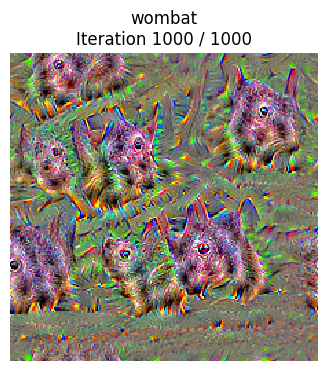
\includegraphics[width=.7\linewidth]{SqueezeNet/wombat_animated_1000_last_frame.png}
        \caption{Last iteration}
        \label{fig:class_viz_wombat:png}
    \end{subfigure}%
    \begin{subfigure}{.5\textwidth}
        \centering
        % \begin{frame}{}
        %     \animategraphics[width=.7\linewidth]{10}{SqueezeNet/wombat_animated_1000/frame-}{0}{999}
        % \end{frame}
        % \includemedia[width=.7\linewidth, height=.7\linewidth]{}{SqueezeNet/wombat_animated_1000.mp4}
        \caption{\href{figs/2b/SqueezeNet/wombat_animated_1000.mp4}{Animation}}
        \label{fig:class_viz_wombat:vid}
    \end{subfigure}
    \caption{Class visualization: started from random noise, maximising the score from the wombat class. Using default regularization parameters (regularization factor of $10^{-3}$, bluring every ten epoch, learning rate of $5$).}
    \label{fig:class_viz_wombat}
\end{figure}

\paragraph*{9. Try to vary the number of iterations and the learning rate as well as the regularization weight.}
To improve class visualization, it appears that regularization and blurring plays a crucial role. In the following figure, we experimented with modifiying the learning rate, the image blurring frequency and the weight regularization on SqueezeNet.% Although we initially used a different model to achieve better visuals, all experiments were subsequently conducted on both SqueezeNet and VGG16.

As a baseline for comparison with upcoming experiments, \Cref{fig:class_viz_baseline} represents the class visualization of the "bee eater" class using the default parameters from the practical implementation, which include a learning rate of $5$, a regularization of $1e^{-3}$, and applying blurring every ten epochs.
\begin{figure}[H]
    \centering
    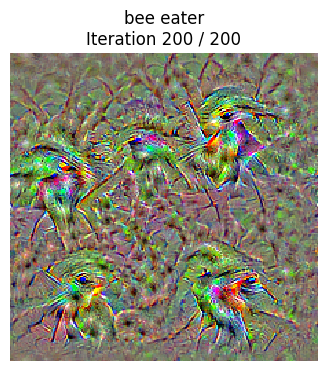
\includegraphics[width=.35\textwidth]{figs_propre2/SqueezeNet/SqueezeNet_bird_animated_last_frame.png}
    \caption{Baseline class visualization for the "bee eater" class, provided here for comparison, was generated using a learning rate of $5$, a regularization strength of $1e^{-3}$, and blurring applied every ten epochs.}
    \label{fig:class_viz_baseline}
\end{figure}%

%%% L2 REG %%%
In our first experiment, we explore the impact of the l2-regularization parameter. As a reminder, the default regularization factor is set to $1e^{-3}$. \Cref{fig:class_viz_reg} presents the results obtained using a $1e^{-5}$ regularization factor for 200 epochs and $1e^{-2}$ regularization factors for 200 and 2000 epochs.

Non-regularized images appear to be overly saturated and noisy, even away from bird figures, making it challenging to discern the represented class clearly. Our suspicion is that without regularization, the image become saturated in \textbf{every pixel} that could have contributed to a correct prediction of the ''bee eater'' class to maximise the class score.

Conversely, when over-regularization is applied, the resulting images appear to have "lighter" class visualizations, even after 2000 epochs. However, the noise in these images remains low and consistent, and the boundaries of the birds are clear and distinguishable. On the downside, the birds themselves appear to be less colorful in these images. By constraining pixel values, we encourage the model to make judicious decisions about which pixels to modify, creating better frontiers.

\begin{figure}[H]
    \centering
    \begin{subfigure}[t]{.33\textwidth}
        \centering
        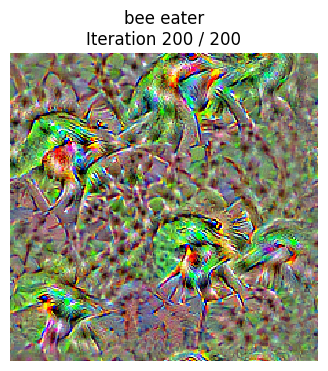
\includegraphics[width=\linewidth]{figs_propre2/SqueezeNet/SqueezeNet_bird_animated_reg_5_last_frame.png}
        \caption{}
        \label{fig:class_viz_reg:sub1}
    \end{subfigure}%
    \begin{subfigure}[t]{.33\textwidth}
        \centering
        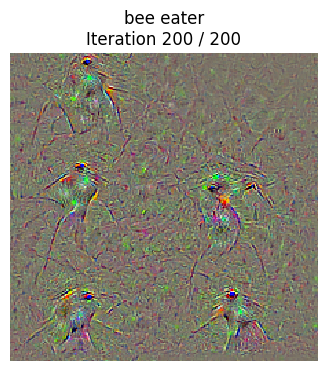
\includegraphics[width=\linewidth]{figs_propre2/SqueezeNet/SqueezeNet_bird_animated_reg_2_last_frame.png}
        \caption{}
        \label{fig:class_viz_reg:sub2}
    \end{subfigure}%
    \begin{subfigure}[t]{.33\textwidth}
        \centering
        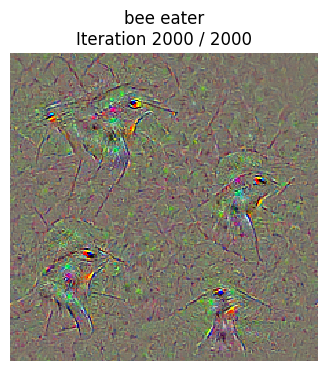
\includegraphics[width=\linewidth]{figs_propre2/SqueezeNet/SqueezeNet_bird_animated_2000_reg_2_last_frame.png}
        \caption{}
        \label{fig:class_viz_reg:sub3}
    \end{subfigure}
    \caption{Comparaison of the bee eater class visualization using SqueezeNet (a) using low regularization ($ 1e^{-5} $), (b) using high regularization ($ 1e^{-2} $). (c) using high regularization ($ 1e^{-2} $) on 2000 epochs} % (blurring and weight regularization) % and starting from a base image of the class.
    \label{fig:class_viz_reg}
\end{figure}


%%% BLUERING %%%
In our second experiment, we focus on modifying the blurring frequency. In the baseline (\Cref{fig:class_viz_baseline}), blurring occurs every ten steps. In \Cref{fig:class_viz_blur}, we explore two variations: blurring every two steps and no blurring at all. The first image represents the baseline (blur every ten epochs), provided here for quick comparison.

The second image, where blurring happens every two steps, showcases birds that are considerably more detailed and clear in our assessment. In contrast to the last image, there are no peculiar patterns extending around the birds.

Blurring appears to prevent the extension of repeated patterns around the visualization. By encouraging pixels that the model has already engaged in transformations and maintaining their direction, blurring facilitates the emergence of a more genuine and detailed class image.

\begin{figure}[H]
    \centering
    \begin{subfigure}[t]{.33\textwidth}
        \centering
        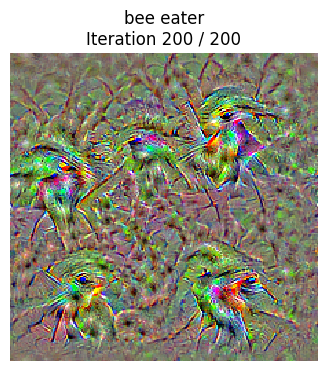
\includegraphics[width=\linewidth]{figs_propre2/SqueezeNet/SqueezeNet_bird_animated_last_frame.png}
        \caption{}
        \label{fig:class_viz_blur:sub1}
    \end{subfigure}%
    \begin{subfigure}[t]{.33\textwidth}
        \centering
        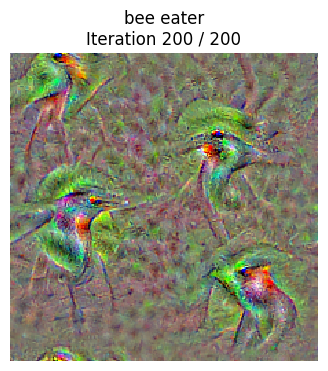
\includegraphics[width=\linewidth]{figs_propre2/SqueezeNet/SqueezeNet_bird_animated_blur++_last_frame.png}
        \caption{}
        \label{fig:class_viz_blur:sub2}
    \end{subfigure}%
    \begin{subfigure}[t]{.33\textwidth}
        \centering
        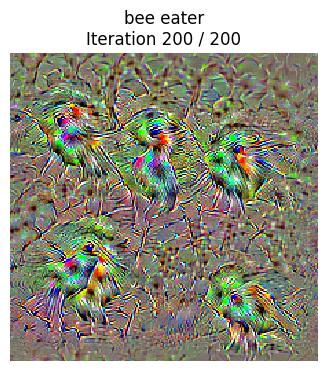
\includegraphics[width=\linewidth]{figs_propre2/SqueezeNet/SqueezeNet_bird_animated_no_blur_last_frame.png}
        \caption{}
        \label{fig:class_viz_blur:sub3}
    \end{subfigure}
    \caption{Comparison of the bee eater class visualization using SqueezeNet: (a) Blurring every ten steps (baseline, provided here for easier comparison). (b) Blurring every two steps. (c) Without blurring.} % (blurring and weight regularization) % and starting from a base image of the class.
    \label{fig:class_viz_blur}
\end{figure}

%%% Epoch number %%%

Regarding the number of epochs, our experiments indicate that a certain number of epochs are needed for the visualization to converge and produce better images. However, it's important to note that as the process continues, the images can become saturated or reach a point where further training may not significantly improve the results. This suggests that there's a trade-off between the number of epochs for convergence and the risk of overfitting or saturation in the generated images.

\begin{figure}[H]
    \centering
    \begin{subfigure}[t]{.25\textwidth}
        \centering
        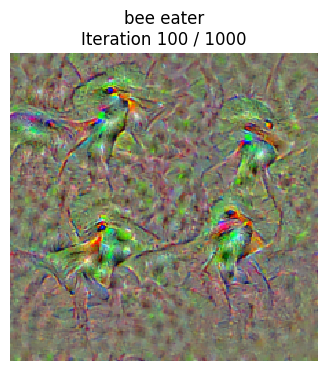
\includegraphics[width=\linewidth]{figs_propre2/SqueezeNet/SqueezeNet_bird_animated_1000_blur_100_frame.png}
        % \caption{200 iterations}
        \caption{}
        \label{fig:class_viz_iter:sub1}
    \end{subfigure}%
    \begin{subfigure}[t]{.25\textwidth}
        \centering
        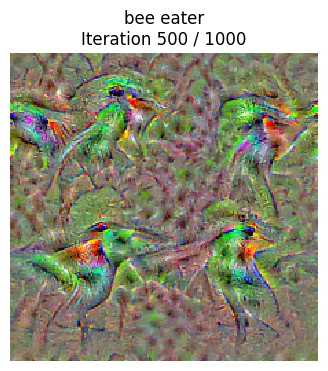
\includegraphics[width=\linewidth]{figs_propre2/SqueezeNet/SqueezeNet_bird_animated_1000_blur_500_frame.png}
        % \caption{500 iterations}
        \caption{}
        \label{fig:class_viz_iter:sub2}
    \end{subfigure}%
    \begin{subfigure}[t]{.25\textwidth}
        \centering
        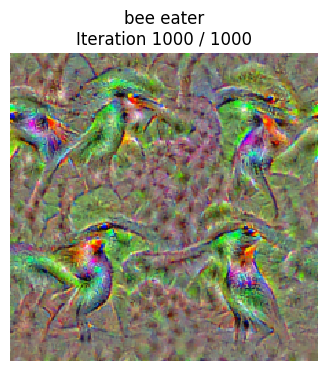
\includegraphics[width=\linewidth]{figs_propre2/SqueezeNet/SqueezeNet_bird_animated_1000_blur_last_frame.png}
        % \caption{1000 iterations}
        \caption{}
        \label{fig:class_viz_iter:sub3}
    \end{subfigure}%
    \begin{subfigure}[t]{.25\textwidth}
        \centering
        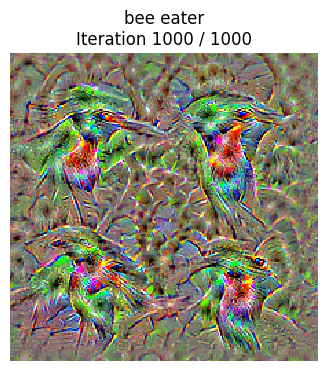
\includegraphics[width=\linewidth]{figs_propre2/SqueezeNet/SqueezeNet_bird_animated_1000_last_frame.png}
        % \caption{1000 iterations, no regularization}
        \caption{}
        \label{fig:class_viz_iter:sub4}
    \end{subfigure}
    \caption{Comparaison of the bee eater class visualization using SqueezeNet with strong regularizations (a) 200 iterations, (b) 500 iterations, (c) 1000 iterations and (d) 1000 iterations without applying regularization.}
    \label{fig:class_viz_iter}
\end{figure}

%%% Learning Rate %%%
About the learning rate, we know from previous courses that it permit a better exploration of loss landscape but modifiy the convergence speed.

We conducted experiments with two variations of the learning rate: 1. Increasing it by a factor of two (from 5 in the baseline to 10). 2. Reducing it by a factor of ten (from 5 in the baseline to 0.5). It's worth noting that reducing the learning rate makes the convergence significantly slower. To compensate for this, we also tried the reduced learning rate setting with 2000 iterations. Results are presented in \Cref{fig:class_viz_lr}.

Using a high learning rate results in images that appear rushed, with a significant amount of noise, and the birds are nearly indistinguishable. On the other hand, with a low learning rate, especially at 2000 steps, the birds seem to merge with the background noise, and patterns appear larger and lighter.

Our observation suggests that a lower learning rate allows for better convergence toward a global minimum, but it may also lead to the model getting trapped in a local minimum, resulting in the dreamlike aspect of the image.

\begin{figure}[H]
    \centering
    \begin{subfigure}[t]{.33\textwidth}
        \centering
        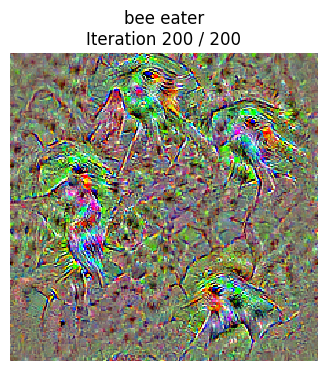
\includegraphics[width=\linewidth]{figs_propre2/SqueezeNet/SqueezeNet_bird_animated_lr_10_last_frame.png}
        \caption{}
        \label{fig:class_viz_lr:sub1}
    \end{subfigure}%
    \begin{subfigure}[t]{.33\textwidth}
        \centering
        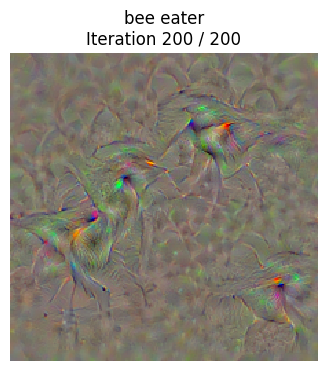
\includegraphics[width=\linewidth]{figs_propre2/SqueezeNet/SqueezeNet_bird_animated_lr_0.5_last_frame.png}
        \caption{}
        \label{fig:class_viz_lr:sub2}
    \end{subfigure}%
    \begin{subfigure}[t]{.33\textwidth}
        \centering
        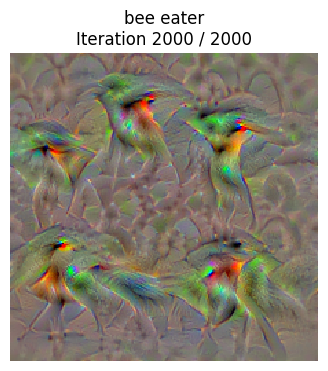
\includegraphics[width=\linewidth]{figs_propre2/SqueezeNet/SqueezeNet_bird_animated_2000_lr_0.5_last_frame.png}
        \caption{}
        \label{fig:class_viz_lr:sub3}
    \end{subfigure}
    \caption{Comparaison of the bee eater class visualization using SqueezeNet (a) } % (blurring and weight regularization) % and starting from a base image of the class.
    \label{fig:class_viz_lr}
\end{figure}

\paragraph*{10. Try to use an image from ImageNet as the source image instead of a random image. You can use the real class as the target class. Comment on the interest of doing this.}

Initiating the process with an image from ImageNet is a valuable approach. It provides a meaningful starting point for gradient-based visualization, ensuring that the initial gradients are directed towards relevant features and patterns within the image. It prevents the initial gradients from scattering or diverging in various directions, potentially resulting in a more focused and interpretable visualization.

\begin{figure}[H]
    \centering
    \begin{subfigure}{.33\textwidth}
        \centering
        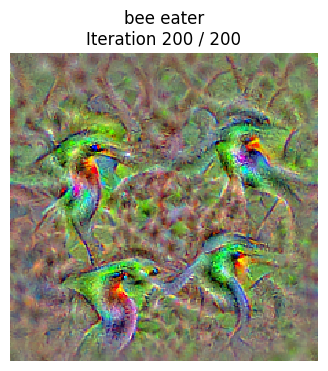
\includegraphics[width=\linewidth]{SqueezeNet/bird_animated_reg++_last_frame.png}
        % \caption{Last iteration\\starting from noise}
        \caption{}
        \label{fig:class_viz_start_image:png_noise}
    \end{subfigure}%
    \begin{subfigure}{.33\textwidth}
        \centering
        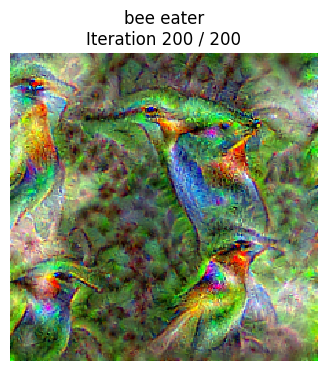
\includegraphics[width=\linewidth]{SqueezeNet/bird_animated_same_init_img_reg++_last_frame.png}
        % \caption{Last iteration\\starting from same class}
        \caption{}
        \label{fig:class_viz_start_image:png}
    \end{subfigure}%
    \begin{subfigure}{.33\textwidth}
        \centering
        % \begin{frame}{}
        %     \animategraphics[width=.7\linewidth]{10}{SqueezeNet/bird_animated_same_init_img_reg++/frame-}{0}{199}
        % \end{frame}
        \caption{\href{figs/2b/bird_animated_same_init_img_reg++.gif}{Animation} starting from same class.} %(see \textit{SqueezeNet\_bird\_animated\_same\_init\_img\_reg++.gif})}
        \label{fig:class_viz_start_image:vid}
    \end{subfigure}
    \caption{Class visualization using SqueezeNet: (a) Last iteration starting from noise, (b) Last iteration starting from the same class, and (c) \href{figs/2b/bird_animated_same_init_img_reg++.gif}{Animation} starting from the same class to maximize the score for the bee eater class, all with high blurring frequency (2) and a sligthly lower regularization ($ 1e^{-5} $ ).}
    \label{fig:class_viz_start_image}
\end{figure}

It pretty funny to create some objects from other objects. In \Cref{fig:class_viz_start_image_dif} we started from a image of hays to do a snail class visualization.

\begin{figure}[H]
    \centering
    \begin{subfigure}{.33\textwidth}
        \centering
        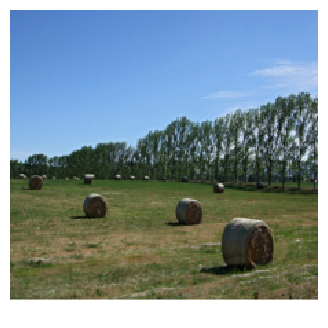
\includegraphics[width=\linewidth]{figs_propre2/hays.png}
        \caption{Original image}
        \label{fig:class_viz_start_image_dif:baseimage}
    \end{subfigure}%
    \begin{subfigure}{.33\textwidth}
        \centering
        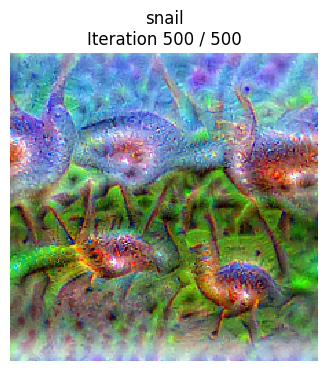
\includegraphics[width=\linewidth]{SqueezeNet/snail_animated_init_img_reg++_last_frame.png}
        \caption{Last iteration}
        \label{fig:class_viz_start_image_dif:png}
    \end{subfigure}%
    \begin{subfigure}{.33\textwidth}
        \centering
        % \begin{frame}{}
        %     \animategraphics[width=\linewidth]{10}{SqueezeNet/snail_animated_init_img_reg++/frame-}{0}{499}
        % \end{frame}
        \caption{\href{figs/2b/SqueezeNet/snail_animated_init_img_reg++.gif}{Animation}}
        \label{fig:class_viz_start_image_dif:vid}
    \end{subfigure}
    \caption{Class visualization using SqueezeNet with strong regularizations: Initiated from an initial hay image, aiming to maximize the score for the snail class.}
    \label{fig:class_viz_start_image_dif}
\end{figure}

\paragraph*{11. \textbf{Bonus:} Test with another network, VGG16, for example, and comment on the results.}
We conducted identical experiments using VGG16 this time. Visualizations are often superior due to VGG16's overall improved performance, as previously discussed in \Cref{paragraph:bonus_VGG}. Specifically, we found the hay to snail animation in \Cref{fig:class_viz_start_image_dif_VGG:vid} to be more appealing. However, there are instances where regularization proves to be more challenging, as observed in \Cref{fig:class_viz_iter_vgg} or when comparing \ref{fig:class_viz_wombat_VGG:b} and \ref{fig:class_viz_wombat_VGG:c}.

\begin{figure}[H]
    \centering
    \begin{subfigure}{.5\textwidth}
        \centering
        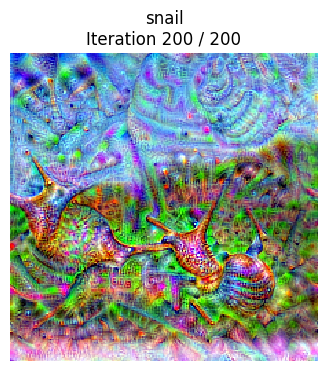
\includegraphics[width=.7\linewidth]{VGG/VGG_snail_animated_init_img_reg++_last_frame.png}
        \caption{Last iteration}
        \label{fig:class_viz_start_image_dif_VGG:png}
    \end{subfigure}%
    \begin{subfigure}{.5\textwidth}
        \centering
        % \begin{frame}{}
        %     \animategraphics[width=.7\linewidth]{10}{VGG/VGG_snail_animated_init_img_reg++/frame-}{0}{499}
        % \end{frame}
        \caption{\href{figs/2b/VGG/VGG_snail_animated_init_img_reg++.gif}{Animation}}
        \label{fig:class_viz_start_image_dif_VGG:vid}
    \end{subfigure}
    \caption{Class visualization using VGG with high blurring frequency (2) and a sligthly lower regularization ($ 1e^{-5} $ ): started from a hay image to maximising the score for the snail class.}
    \label{fig:class_viz_start_image_dif_VGG}
\end{figure}

\begin{figure}[H]
    \centering
    \begin{subfigure}[t]{.25\textwidth}
        \centering
        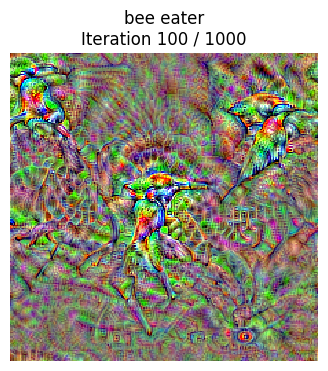
\includegraphics[width=\linewidth]{VGG/VGG_bird_animated_1000_regpp_blur_100_frame.png}
        % \caption{200 iterations}
        \caption{}
        \label{fig:class_viz_iter_vgg:sub1}
    \end{subfigure}%
    \begin{subfigure}[t]{.25\textwidth}
        \centering
        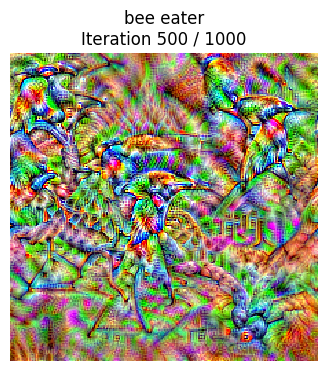
\includegraphics[width=\linewidth]{VGG/VGG_bird_animated_1000_regpp_blur_500_frame.png}
        % \caption{500 iterations}
        \caption{}
        \label{fig:class_viz_iter_vgg:sub2}
    \end{subfigure}%
    \begin{subfigure}[t]{.25\textwidth}
        \centering
        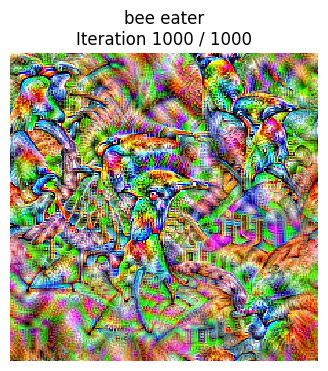
\includegraphics[width=\linewidth]{VGG/VGG_bird_animated_1000_regpp_blur_last_frame.png}
        % \caption{1000 iterations}
        \caption{}
        \label{fig:class_viz_iter_vgg:sub3}
    \end{subfigure}%
    \begin{subfigure}[t]{.25\textwidth}
        \centering
        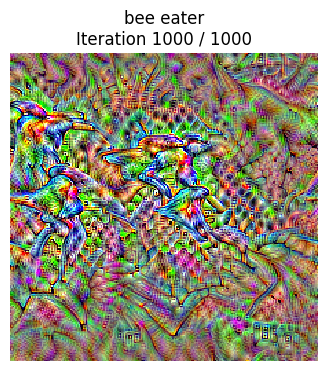
\includegraphics[width=\linewidth]{VGG/VGG_bird_animated_1000_last_frame.png}
        % \caption{1000 iterations, no regularization}
        \caption{}
        \label{fig:class_viz_iter_vgg:sub4}
    \end{subfigure}
    \caption{Comparaison of the bee eater class visualization using VGG with with high blurring frequency (2) and a sligthly lower regularization ($ 1e^{-5} $ ) (a) 200 iterations, (b) 500 iterations, (c) 1000 iterations and (d) at 1000 iterations but without having performed regularization.}
    \label{fig:class_viz_iter_vgg}
\end{figure}

\begin{figure}[H]
    \centering
    \begin{subfigure}{.32\textwidth}
        \centering
        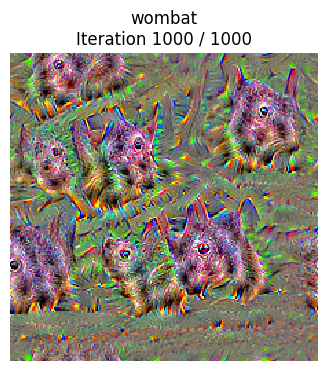
\includegraphics[width=\linewidth]{SqueezeNet/wombat_animated_1000_last_frame.png}
        \caption{}
        \label{fig:class_viz_wombat_VGG:a}
    \end{subfigure}%
    \begin{subfigure}{.32\textwidth}
        \centering
        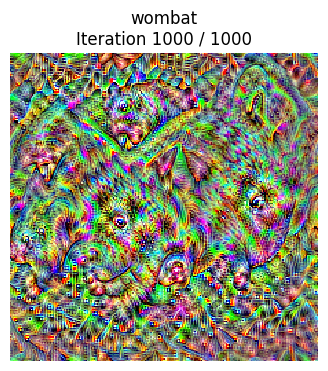
\includegraphics[width=\linewidth]{VGG/VGG_wombat_animated_1000_last_frame.png}
        \caption{}
        \label{fig:class_viz_wombat_VGG:b}
    \end{subfigure}%
    \begin{subfigure}{.32\textwidth}
        \centering
        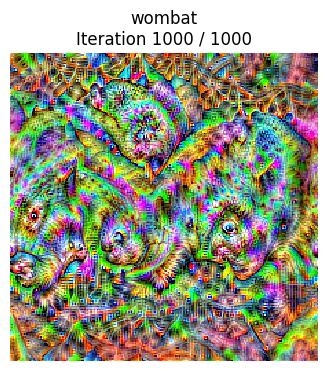
\includegraphics[width=\linewidth]{VGG/VGG_wombat_animated_1000_regpp_blur_last_frame.png}
        \caption{}
        \label{fig:class_viz_wombat_VGG:c}
    \end{subfigure}
    \caption{Class visualization of Wombat. (a) Using SqueezeNet for comparison with default parameters; (b) Using VGG with default parameters; (c) Using VGG with high blurring frequency (2) and a sligthly lower regularization ($ 1e^{-5} $ ).}
    \label{fig:class_viz_wombat_VGG}
    %TODO Ici j'trouve les figures plus mitigé qu'avec squeeze net, j'ai envie de mettre celle de squeeze net pour une comparaison plus directe 
\end{figure}

